\pdfoutput=1

\documentclass[preprint,12pt,authoryear]{elsarticle}

\usepackage{amsmath,amssymb,amsfonts}
\usepackage{amsthm}
\journal{Journal of Mathematical Psychology}

\theoremstyle{plain}
\newtheorem{theorem}{Theorem}[section]
\newtheorem{proposition}[theorem]{Proposition}
\newtheorem{lemma}[theorem]{Lemma}
\newtheorem{corollary}[theorem]{Corollary}
\newtheorem{conjecture}[theorem]{Conjecture}
\theoremstyle{definition}
\newtheorem{definition}[theorem]{Definition}
\theoremstyle{remark}
\newtheorem{remark}[theorem]{Remark}

\usepackage{microtype}
\usepackage{xcolor}
\usepackage{booktabs}
\usepackage{tikz}
\usepackage{mathtools}
\usetikzlibrary{arrows.meta,positioning,calc,decorations.pathreplacing}
\usepackage{hyperref}
\hypersetup{hidelinks}
\usepackage[nameinlink,capitalise]{cleveref}

%% Line numbers for the review version (uncomment \linenumbers below if desired)
\usepackage{lineno}

%%%% Basic macros
\newcommand{\Real}{\mathbb{R}}
\newcommand{\Complex}{\mathbb{C}}
\newcommand{\Sphere}{\mathbb{S}}
\newcommand{\Hue}{S^{1}}
\newcommand{\Lscale}{\kappa}
\DeclareMathOperator{\spec}{spec}

%% Target journal (appears in preprint header)
\journal{Journal of Mathematical Psychology}

\begin{document}

\begin{frontmatter}

\title{The Magenta Gap: A Geometric Reachability Model of Nonspectral Hue and Color Gamut Boundaries}

\author[ao]{Alexander Yiannopoulos\corref{cor1}}
\ead{ayianno@ao.institute}
\cortext[cor1]{Corresponding author}
\address[ao]{A$\lvert\Omega\rangle$ Institute, Alpha Omega Lattice Corporation\\3724 Laurel Street, Suite 108, New Orleans, Louisiana, USA}

\end{frontmatter}

\section{Introduction}
\label{sec:introduction}

\noindent Color perception provides a concrete test case for a fundamental question in mathematical psychology: how does an embodied visual system transform an ordered physical stimulus domain---the physical electromagnetic spectrum---into a phenomenal space governed by different topology, metric structure, and reachability constraints? The geometric study of color perception along these lines is well-established. Differential-geometric models of color space originate with \citet{Schrodinger1920} and were placed on a rigorous footing by \citet{Resnikoff1974}, and the metric structure of perceptual color continues to be actively revised \citep{Bujack2022}. Our treatment departs from the preceding tradition in two key respects: it foregrounds the \emph{topology} of hue closure before any metric is imposed, and it interprets the metric of the color body as a reachability gauge rather than a perceptual-distance metric.

The central claim of this paper is that the transformation from physical stimulus to phenomenal color does \emph{not} preserve topology, metric geometry, or reachability relations. The supporting claims advanced below have different statuses. The compactification argument is a topological analysis of the mismatch between the ordered monochromatic locus and cyclic phenomenal hue. The resolved seam and achromatic quotient are proposed as structural models of the phenomenal target space. The Lorentzian spindle model is a calibrated kinematic normal form for reachability; its role is to represent the boundary between ordinary optical accessibility and chimerical access under altered visual operating conditions. By treating phenomenal color space as an invariant geometric construction rather than a passive reflection of physical light, the paper formulates nonspectral hue and color-gamut boundaries as a formal boundary-value problem in the geometry of perception.

In brief: let $\mathcal{S}_a$ denote the infinite-dimensional space of admissible finite positive spectral measures, representing spectral power distributions capable of stimulating an observer or visual regime $a$. Restricted to the idealized monochromatic locus of an organism-relative visible range, the physical electromagnetic spectrum may be represented as an open interval: a bounded 1-manifold embedded in the real continuum $\mathbb{R}$. This is the familiar ``rainbow spectrum.'' Conversely, however, phenomenal hue is experienced as periodic, forming a closed 1-sphere $S^1$---the familiar ``color wheel.'' On a linear rainbow spectrum, every path from red to violet passes through green. On a circular color wheel, however, a second route exists: hue closes from violet back to red through the nonspectral purples, never re-traversing green.

This closure mechanism is the source of the ``magenta gap.'' Magenta corresponds to no single wavelength; it is the psychophysical response induced by combinations of wavelengths near opposing endpoints of an observer's visible range. Because the physical interval is open while the hue manifold is closed, the response-side geometry must represent a closure in order to produce a continuous, periodic hue space. Abstractly, this transition is modeled by a one-point compactification, adjoining a single closure point to the open spectral interval $I_a$ to form a circle $H_a\cong S^1$. However, phenomenal experience does not traverse this closure as a dimensionless singularity. The visual system resolves the abstract closure point into a macroscopic continuum of distinguishable nonspectral purples.

Formally, we model this resolution by a continuous map
\[
\pi:\widetilde{H}_a\longrightarrow H_a,
\]
where $\widetilde{H}_a$ represents the resolved phenomenal hue space, $\pi$ is a diffeomorphism away from the closure seam, and the exceptional fiber over the seam is
\[
\pi^{-1}(\infty)\cong [0,1].
\]
This exceptional fiber is the line of purples. In an operational human-observer implementation, the limiting short- and long-wavelength directions may be approximated by finite sampling values such as 390 nm and 700 nm. These values should not be identified with elements of the open physical interval \(I_a\) itself. Rather, they represent finite experimental proxies for the ideal boundary directions \(\lambda_-^a\) and \(\lambda_+^a\) in the auxiliary closure \(\overline I_a=[\lambda_-^a,\lambda_+^a]\). The purple fiber is therefore attached in the response-side resolved hue space, not by adding new wavelengths to the physical spectral interval. The magenta gap is not a missing physical wavelength, but a response-side topological bridge resolving the abstract closure of phenomenal hue.

Fixing the topology of hue, however, does not determine the metric of the full color gamut. Globally, the idealized phenomenal color body is a solid three-dimensional space with an achromatic axis. In cylindrical chromatic coordinates, it must be rigorously defined as the quotient
\[
M_a \cong \bigl([0,R_a]\times \widetilde{H}_a\times L_a\bigr)/{\sim},
\]
where $L_a\subset\mathbb{R}$ denotes the luminosity range and $(0,\theta,z)\sim(0,\theta',z)$ for all hue angles $\theta,\theta'$ and all $z\in L_a$. This quotient expresses the fundamental phenomenological fact that hue is undefined at absolute zero saturation.

At the achromatic axis $A_a=\{r=0\}$ the hue coordinate degenerates. For the metric to remain well defined there, the angular coordinate must be normalized so that the chromatic plane $dr^2+r^2\,d\theta^2$ closes without a conical defect; this normalization is made explicit in \Cref{sec:compactification}.

On the chromatic stratum $M_a^{\ast}=M_a\setminus A_a$, the hue projection defines a trivial bundle $M_a^{\ast}\longrightarrow S^1$ with local fiber coordinates $(r,z)$. Each fixed hue determines a radial--luminosity section carrying a pseudo-Riemannian metric of signature $(1,1)$. In cylindrical chromatic coordinates, the local metric may be written
\[
g = dr^2 + r^2\,d\theta^2 - \kappa^2\,dz^2,
\]
where $\theta$ is hue, $r$ is saturation, $z$ is luminosity, and $\kappa>0$ fixes the relative scale of luminosity displacement.

The signature is not arbitrary. Luminosity is the distinguished (timelike) coordinate because the reachability structure developed below is organized along the luminosity axis: its two poles are the achromatic extremes of luminosity, and the boundary of the reachable color body is the cone structure encoding accessibility between them. The minus sign on $dz^2$ thus records the role of luminosity as the axis of reachability, not a claim that luminosity differences are subjectively imaginary.

The essential role of the indefinite metric becomes clearest when formalizing the boundary structure of the color spindle \citep{Churchland2005}. The spindle distinguishes ordinary colors, which are induced by continuous visual input, from chimerical or impossible colors, which lie outside the familiar range of stimulus-accessible color experience. Chimerical colors are empirically reproducible phenomenal states---reddish green and yellowish blue have been reported under retinal-image stabilization that fatigues opponent channels \citep{CranePiantanida1983}---but they are reached through altered operating conditions of the visual system rather than by continuous variation of ordinary optical input alone.

To make this distinction precise, let $a_0$ denote a normal visual operating regime. The ordinary optical response map is modeled as a smooth response map from the physical stimulus space into the phenomenal manifold:
\[
\Phi_{a_0}:\mathcal{S}_{\mathrm{ord}}^{a_0} \longrightarrow M_{a_0}.
\]
Defining the ordinary color spindle as its image, $C_{a_0} := \operatorname{im}(\Phi_{a_0}) \subset M_{a_0}$, we model this restricted phenomenal space as a \textit{kinematic reachability body} bounded by a piecewise null hypersurface.

At first glance, importing indefinite pseudo-Riemannian geometry into a model of color perception may appear counterintuitive. The analogy, however, is limited and specific. The metric is not introduced as a perceptual distance metric. It is introduced as a \textit{kinematic reachability gauge}: a formal device for representing the boundary between states reachable by continuous optical variation under a fixed operating regime and states accessible only after alteration of that regime. A null boundary provides no confinement if arbitrary spacelike transitions are allowed. The restriction of the spindle is therefore not merely a static feature of the metric, but a dynamic constraint on the control fields generated by the visual response map. In this model, chimerical colors are represented as exterior states because they cannot be reached by continuous optical variation alone; they require a change in the ordinary visual operating regime, such as opponent-channel fatigue.

In the idealized symmetric case this reachability body takes a simple closed form. With a single constant luminosity scale and centered achromatic poles at the two extremes of luminosity, the locus on which chromatic displacement exactly balances luminosity displacement is a bicone: two null cones meeting in a $C^0$ ridge at the isoluminant equator. \Cref{sec:reachability} constructs this normal form explicitly, verifies that its boundary generators are null, and develops the empirically calibrated, hue-dependent deformation that replaces the constant scale with a saturation ceiling varying around the hue circle.

This normal form yields a falsifiable structural prediction. If the spindle boundary is the piecewise null reachability envelope previewed here, then empirical color solids should exhibit a genuine $C^0$ non-differentiability---a ridge---at the isoluminant equator, and this ridge should be a robust structural feature rather than measurement noise to be smoothed away. In operational psychophysics, non-differentiable ridges in measured color solids are often treated as artifacts and removed by higher-order approximations. The present model predicts where such a ridge should occur and identifies it as part of the calibrated normal form. To be clear, this is not a general prohibition on smoothing empirical data; rather, it is a specific, testable claim about the shape of measured gamut boundaries when the boundary is interpreted as a \textit{kinematic reachability horizon}.

The same construction yields a second, quantitative consequence. Requiring the deformed boundary to remain null forces a coordinate-invariant admissibility bound relating the hue-dependent saturation ceiling to the local discrimination geometry. The human gamut is shown to satisfy this bound---and to violate its naive coordinate-dependent counterpart---when evaluated against the Stockman--Sharpe cone fundamentals, with the MacAdam discrimination ellipses providing an independent consistency check (\ref{app:numerics}).

The remainder of the paper develops this construction in three steps: first, the compactification and response-side resolution of hue; second, the quotient and local metric structure of the vivid color body; and third, the reachability envelope and the local boundary constraint it imposes. By mapping the phenomenal color manifold in these geometric terms, the explanatory target is made concrete: it becomes the problem of specifying the structural non-isomorphism by which an embodied visual system transforms a physical stimulus manifold into a phenomenal geometry with its own topology, metric structure, and reachability constraints.


%%%%%%%%%%%%%%%%%%%%%%%%%%%%%%%%%%%%%%%%%%%%%%%%%%%%%%%%%%%%%%%%%%%%%%%%%%
%%% SECTION 2: THE MAGENTA GAP
%%%%%%%%%%%%%%%%%%%%%%%%%%%%%%%%%%%%%%%%%%%%%%%%%%%%%%%%%%%%%%%%%%%%%%%%%%
\section{The Magenta Gap}
\label{sec:magenta-gap}

\noindent Magenta has no monochromatic physical correlate. It is a robust and reproducible phenomenal response to physically real spectral power distributions, but it is not parameterized by any one single wavelength of light. Magenta is a color generated by the visual system when two physically distinct regions of the electromagnetic spectrum jointly stimulate an appropriately-situated observer. Magenta is therefore physically induced, but strictly nonspectral.

\subsection{Spectral stimuli and phenomenal hue}
\label{subsec:spectral-stimuli-phenomenal-hue}

\noindent A physical description of light specifies wavelength, frequency, intensity, polarization, or spectral power distribution. None of these quantities is, in itself, a phenomenal hue. Wavelength does not contain redness, greenness, or violetness as an intrinsic physical property. Rather, wavelengths produce color appearances only through their interaction with a visual system. This point is standard in color science: the appearance of color depends on the relation between physical stimulation, photoreceptor sensitivities, opponent processing, adaptation state, and neural interpretation \citep{Shevell2003,Hardin1988,Thompson1995}.

It is nevertheless useful to speak operationally of spectral colors. A spectral color is a phenomenal hue that can be induced, under suitable conditions, by approximately monochromatic light. In this operational sense, a narrow-band stimulus near one end of the human visible range may appear violet, while a narrow-band stimulus near the other end may appear red. This does not identify hue with wavelength; it identifies a restricted class of phenomenal responses reliably induced by a restricted class of physical stimuli.

The distinction matters because the physical wavelength parameter is linearly ordered, while phenomenal hue is not. Moving through monochromatic wavelengths from the short-wavelength region to the long-wavelength region produces a familiar sequence of spectral appearances. But phenomenal hue does not terminate at those two spectral regions. In ordinary color experience, the red and violet limiting classes are identified through the nonspectral purples. For chromatic colors, hue closes.

\subsection{Nonspectral purples}
\label{subsec:nonspectral-purples}

\noindent The purples occupy the crucial region where the linear spectral ordering fails to capture phenomenal organization. A purple or magenta percept is not produced by a single wavelength lying ``between'' red and violet on the physical spectrum. Physically, that is to say, the wavelengths between the red and violet regions pass through the greens and yellows: the spectrum is linearly ordered by wavelength, from the short-wavelength violet limit (toward the ultraviolet) to the long-wavelength red limit (toward the infrared), with the greens and yellows in between. Phenomenally, however, red and violet are adjacent through purple. The color wheel records this fact at the level of chromatic organization: the two limiting classes of the spectral interval are glued in phenomenal hue space, even though they remain separated in the physical wavelength ordering.

This is an ordinary operational feature of visual organization. Magenta is induced by spectral power distributions that jointly stimulate regions near opposite ends of an observer's visible range. In human vision, such stimuli typically involve energy in long-wavelength and short-wavelength regions, with suppressed contribution from the middle wavelengths associated with greenish appearances. The resulting percept is experienced not as a disordered mixture of red and violet, but as a determinate hue with its own phenomenal character.

This clarifies the formal limitation of any account that identifies color too directly with a coordinate on the physical spectrum. Sophisticated physicalist accounts appeal to surface spectral reflectance, spectral power distribution, or visual-system response profiles \citep{ByrneHilbert2003}. But such accounts must structurally explain why a linearly ordered physical stimulus domain maps onto a phenomenal hue space in which the two limiting spectral classes are literally identified. The magenta gap is not an objection to physical causation; it is a strict topological constraint on the psychophysical map.

\subsection{Observer-relative closure}
\label{subsec:observer-relative-closure}

\noindent The magenta gap is not fixed at a universal pair of physical wavelengths. It depends on the organism and on the relevant visual regime. Human color vision samples only a small portion of the electromagnetic continuum through a specific arrangement of photoreceptor sensitivities and opponent channels. Other organisms sample different domains and organize them differently.

Bee color vision provides a rigorous structural comparison. Honeybees are sensitive to ultraviolet wavelengths invisible to normal human observers. The color often discussed as ``bee-purple'' is induced by combinations involving ultraviolet and longer-wavelength stimulation, functioning as a nonspectral analogue of human purple without corresponding to human magenta in physical wavelength terms \citep{Thompson1995,Lunau2018}. A flower presenting one chromatic pattern to a human visual system may present a fundamentally different topological identification to a bee under identical illumination.

The point is not that bees literally experience human magenta; they do not. The point is that any visual system that constructs a complete, cyclic hue space from a bounded, linearly ordered physical spectral range must exhibit a nonspectral endpoint identification. Human magenta and bee-purple are generated by distinct physical boundary regions. What is invariant is not the physical location of the limits, but their structural role: phenomenal hue identifies regions that remain separated at opposite limiting regions of the physical spectral ordering.

\subsection{The operational magenta gap}
\label{subsec:operational-magenta-gap}

\noindent We may now state the magenta gap operationally. Let $a$ denote a visual regime: an organism, photoreceptor structure, adaptation state, and ordinary operating condition. Let $\mathcal{S}_a$ denote the infinite-dimensional space of finite positive Radon measures (or simply ``spectral measures'') on the physical electromagnetic spectrum, representing all admissible spectral power distributions for regime $a$. This measure-theoretic definition rigorously accommodates both continuous macroscopic light sources and their idealized monochromatic limits. The 1-dimensional interval $I_a$ is formally bridged to $\mathcal{S}_a$ via a specific embedding: the \emph{monochromatic locus}. For any wavelength $\lambda \in I_a$, we assign the idealized Dirac measure $\sigma_\lambda(\omega) \propto \delta(\omega - \lambda)$. Thus, $I_a$ is strictly defined as the 1-dimensional parameterization of this embedded locus within the broader measure space $\mathcal{S}_a$. Let
\[
\Phi_{a}:\mathcal{S}_{a}\longrightarrow M_{a}
\]
denote the corresponding visual response map from the full space of admissible physical spectral measures to the phenomenal color space of that regime.

Let $\epsilon>0$ be sufficiently small that the two collars remain disjoint, and define the one-sided endpoint collars within the parameter space $I_a$:
$$
V_-^{a}(\epsilon)=(\lambda_-^{a},\lambda_-^{a}+\epsilon),
\qquad
V_+^{a}(\epsilon)=(\lambda_+^{a}-\epsilon,\lambda_+^{a}).
$$
These are one-sided collars within $I_a$ whose closures approach the ideal boundary points $\lambda_\pm^a$, which do not themselves belong to the open interval $I_a$. In the functional space $\mathcal{S}_a$, we define the spectral boundary collars $\mathbf{V}_-^a$ and $\mathbf{V}_+^a$ as the subspaces of spectral power distributions whose dominant power integral is strictly localized to $V_-^{a}$ and $V_+^{a}$, respectively. A magenta-type percept for the regime $a$ is induced, paradigmatically, by distributions $\sigma \in \mathcal{S}_a$ with sufficiently strong joint contributions from both functional collars relative to the middle region of $I_a$.

The physical parameter space $I_a$ remains linearly ordered. Its two ideal ends are never physically adjacent. The phenomenal hue manifold, however, identifies these two ideal endpoint directions by one-point compactification:
$$
H_a=\widehat{I}_a=I_a\cup\{\infty\}\cong S^1.
$$
Equivalently, using the closure $\overline I_a=[\lambda_-^a,\lambda_+^a]$ as an auxiliary topological model:
$$
\widehat{I}_a\cong \overline I_a/(\lambda_-^a\sim\lambda_+^a).
$$
This is the minimal topological content of the magenta gap. It is a strictly formal closure: phenomenal hue identifies the two ideal ends of the organism-relative spectral interval.

The colorimetric refinement is that visual systems do not merely identify the two ideal ends; they phenomenally resolve this topological closure into a distinguishable continuum. The single compactification point $\infty$ is resolved---via the seam-resolution construction defined in \Cref{sec:compactification}---into an exceptional fiber
$$
\pi^{-1}(\infty)\cong[0,1]
$$
representing the line of purples.

Importantly, the physical-to-phenomenal map $\Phi_a$ is highly non-injective, inducing a metameric equivalence relation on the stimulus space:
\[
  \sigma_1 \sim_{\mathrm{metamer}} \sigma_2
  \quad \Longleftrightarrow \quad
  \Phi_a(\sigma_1)=\Phi_a(\sigma_2).
\]
Let
\[
  q:\mathcal S_a \longrightarrow \mathcal S_a/{\sim_{\mathrm{metamer}}}
\]
denote the quotient map, and let
\[
  \mathcal M_a^{\mathrm{mono}}
  =
  \{\sigma_\lambda:\lambda\in I_a\}
\]
be the idealized monochromatic locus. Relative to $\Phi_a$, nonspectrality then admits a precise mathematical definition. A spectral hue corresponds to a metameric class whose quotient representative lies in $q(\mathcal M_a^{\mathrm{mono}})$; equivalently, the class contains at least one idealized Dirac stimulus $\sigma_\lambda$. By contrast, the metameric classes corresponding to the purples contain no such Dirac stimulus. The line of purples is therefore represented by a continuous response-side subset of $\mathcal S_a/{\sim_{\mathrm{metamer}}}$ that is disjoint from $q(\mathcal M_a^{\mathrm{mono}})$. Because this subset cannot be coordinatized by any $\lambda\in I_a$, the continuum coordinate $\tau\in[0,1]$ along the closure seam must be parameterized on the response side---reflecting the physiological co-activation of opposing opponent-channel poles---rather than by the physical spectrum itself.

The additive structure of color matching on the stimulus side is classically axiomatized by Grassmann's laws, given a representation-theoretic foundation by \citet{Krantz1975}. That tradition characterizes when stimuli match; it does not fix the geometry of the resulting phenomenal arrangement. The metameric equivalence relation introduced here inherits that matching structure but concerns what it leaves open---the topology and metric of the response-side color body into which matched stimuli are mapped.

\Cref{sec:compactification} formalizes this structural mapping. The organism-relative spectral interval serves as an open physical input domain, the circular organization of hue acts as its one-point compactification, and the purples serve as the colorimetric resolution of the resulting compactification point. \Cref{fig:magenta-gap} summarizes this compactification-and-resolution construction.

\begin{figure}[t]
\centering
\resizebox{\linewidth}{!}{%
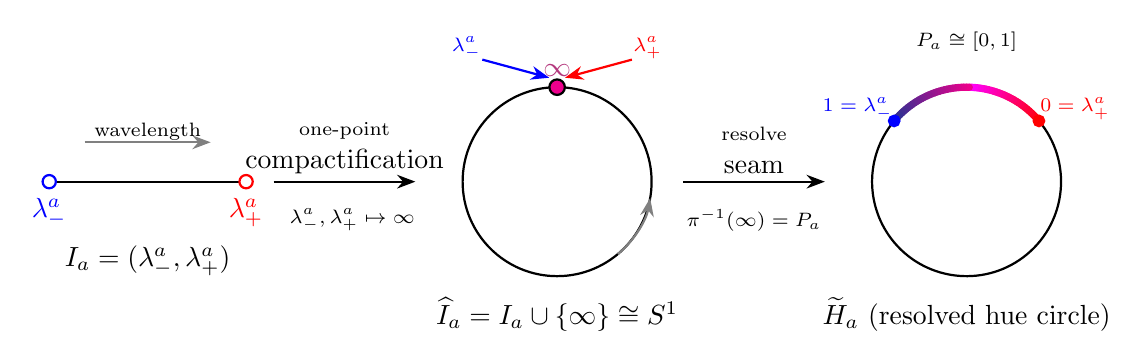
\begin{tikzpicture}[>=Stealth, line width=0.8pt, every node/.style={inner sep=1.5pt}]

  \begin{scope}[shift={(0,0)}]
    \draw (-1.25,0) -- (1.25,0);
    \draw[blue, fill=white] (-1.25,0) circle (2.4pt);
    \draw[red,  fill=white] ( 1.25,0) circle (2.4pt);
    \node[below=4pt, blue] at (-1.25,0) {$\lambda_-^a$};
    \node[below=4pt, red ] at ( 1.25,0) {$\lambda_+^a$};
    \draw[->, gray] (-0.8,0.5) -- (0.8,0.5)
      node[midway, above=-1pt, black] {\scriptsize wavelength};
    \node[anchor=north] at (0,-0.75) {$I_a=(\lambda_-^a,\lambda_+^a)$};
  \end{scope}

  \draw[->] (1.6,0) -- (3.4,0)
    node[midway, above=1pt, align=center] {\scriptsize one-point\\ compactification};
  \node[align=center, anchor=north] at (2.6,-0.28) {\scriptsize $\lambda_-^a,\lambda_+^a \mapsto \infty$};

  \begin{scope}[shift={(5.2,0)}]
    \draw (0,0) circle (1.2);
    \filldraw[draw=black, fill=magenta] (90:1.2) circle (2.8pt);
    \node[above=2pt, magenta!70!black] at (90:1.2) {$\infty$};
    \node[blue] at (-1.15,1.7) {\scriptsize $\lambda_-^a$};
    \node[red ] at ( 1.15,1.7) {\scriptsize $\lambda_+^a$};
    \draw[->, blue] (-0.95,1.55) -- (-0.1,1.32);
    \draw[->, red ] ( 0.95,1.55) -- ( 0.1,1.32);
    \draw[->, gray] (310:1.2) arc (310:350:1.2);
    \node[anchor=north] at (0,-1.4) {$\widehat{I}_a = I_a \cup \{\infty\} \cong S^1$};
  \end{scope}

  \draw[->] (6.8,0) -- (8.6,0)
    node[midway, above=1pt, align=center] {\scriptsize resolve\\ seam};
  \node[align=center, anchor=north] at (7.7,-0.28) {\scriptsize $\pi^{-1}(\infty)=P_a$};

  \begin{scope}[shift={(10.4,0)}]
    \draw (40:1.2) arc (40:-220:1.2);
    \foreach \k in {0,...,29}{
    \pgfmathsetmacro{\a}{40+50*\k/30}
    \pgfmathsetmacro{\b}{40+50*(\k+1)/30}
    \pgfmathtruncatemacro{\p}{100*(29-\k)/29}
    \draw[red!\p!magenta, line width=2.6pt, line cap=round] (\a:1.2) arc (\a:\b:1.2);
  }
  \foreach \k in {0,...,29}{
    \pgfmathsetmacro{\a}{90+50*\k/30}
    \pgfmathsetmacro{\b}{90+50*(\k+1)/30}
    \pgfmathtruncatemacro{\p}{100*(29-\k)/29}
    \draw[magenta!\p!blue, line width=2.6pt, line cap=round] (\a:1.2) arc (\a:\b:1.2);
  }
    \filldraw[red ] ( 40:1.2) circle (1.9pt);
    \filldraw[blue] (140:1.2) circle (1.9pt);
    \node[above left=-2pt,  blue] at (140:1.2) {\scriptsize $1=\lambda_-^a$};
    \node[above right=-2pt, red ] at ( 40:1.2) {\scriptsize $0=\lambda_+^a$};
    \node at (90:1.78) {\scriptsize $P_a \cong [0,1]$};
    \node[anchor=north] at (0,-1.4) {$\widetilde{H}_a$ (resolved hue circle)};
  \end{scope}

\end{tikzpicture}%
}
\caption{The magenta gap as compactification and resolution.
\textbf{(a)} The organism-relative spectrum is an open, linearly ordered
interval $I_a=(\lambda_-^a,\lambda_+^a)$.
\textbf{(b)} Phenomenal hue identifies the two ideal endpoints at a single
point $\infty$, giving the one-point compactification $\widehat{I}_a\cong S^1$.
\textbf{(c)} The seam $\infty$ is resolved into the line of purples
$P_a\cong[0,1]$ (glued with $0\leftrightarrow\lambda_+^a$ and
$1\leftrightarrow\lambda_-^a$), yielding the resolved hue circle
$\widetilde{H}_a$. Spectral ends are colored by wavelength
($\lambda_+^a$ long, red; $\lambda_-^a$ short, blue), and the line of
purples interpolates red--magenta--blue between them. The purples are
nonspectral but not nonphysical: no monochromatic stimulus lies on $P_a$,
yet $P_a$ completes the cyclic structure of hue.}
\label{fig:magenta-gap}
\end{figure}


%%%%%%%%%%%%%%%%%%%%%%%%%%%%%%%%%%%%%%%%%%%%%%%%%%%%%%%%%%%%%%%%%%%%%%%%%%
%%% SECTION 3: COMPACTIFICATION AND RESOLUTION
%%%%%%%%%%%%%%%%%%%%%%%%%%%%%%%%%%%%%%%%%%%%%%%%%%%%%%%%%%%%%%%%%%%%%%%%%%
\section{Compactification and Resolution}
\label{sec:compactification}

\noindent Section~\ref{sec:magenta-gap} established the operational constraint: the organism-relative physical spectrum is linearly ordered, while phenomenal hue is cyclic. The present section formalizes that mismatch. The construction proceeds in two stages. First, the open physical interval is compactified into an abstract hue circle. Second, the single compactification point is resolved into the line of purples. The first operation captures the closure of hue; the second captures the fact that this closure is phenomenally structured.

Let
\[
I_a=(\lambda_-^a,\lambda_+^a)
\]
be the organism-relative open spectral interval associated with visual regime $a$. The values $\lambda_-^a$ and $\lambda_+^a$ are ideal boundary values, not elements of $I_a$. They represent limiting directions approached by the sensitivity profile of the visual system. As a physical stimulus domain, $I_a$ remains linearly ordered. There is no physical adjacency between its two ideal ends.

The abstract hue circle is obtained by one-point compactification:
\[
\widehat I_a=I_a\cup\{\infty\}\cong S^1.
\]
Since $I_a$ is homeomorphic to $\mathbb{R}$, its one-point compactification is unique up to homeomorphism. This is the minimal compactification: it adds exactly one point, which is why the abstract topological closure contains one seam rather than a family of seams.

We write
\[
H_a:=\widehat I_a
\]
for the compactified hue manifold. The added point $\infty$ is the formal closure seam of hue. It is not a wavelength, and it is not an additional physical stimulus. It is the point introduced by the phenomenal organization of hue when the two ideal ends of the organism-relative spectral interval are identified.

Equivalently, using the auxiliary closure $\overline I_a=[\lambda_-^a,\lambda_+^a]$, one may represent the same compactification as the quotient
\[
\widehat I_a\cong \overline I_a/(\lambda_-^a\sim\lambda_+^a).
\]
This quotient representation is only an auxiliary model. The physical stimulus domain remains the open interval $I_a$. The quotient expresses the topological fact that phenomenal hue identifies the two ideal endpoint directions of that interval.

\subsection{Dimensional reduction and the monochromatic locus}
\label{subsec:dimensional-reduction}

\noindent Before executing the topological closure, we must formally bridge the infinite-dimensional physical stimulus domain and the idealized 1-manifold $I_a$. The full domain of admissible physical inputs, $\mathcal{S}_a$, is the infinite-dimensional space of finite positive Radon measures, representing all admissible spectral power distributions. The visual response map $\Phi_a$ does not operate on this space as a direct identity; rather, it executes a massive dimensional reduction by integrating these power distributions against a finite set of broadly tuned photoreceptor sensitivities.

This projection from $\mathcal{S}_a$ into a finite-dimensional physiological excitation space is fundamentally non-injective, establishing the mathematical basis of chromatic metamerism. Within this smooth physiological excitation space, the biological responses to purely monochromatic Dirac measures $\sigma_\lambda\propto\delta(\omega-\lambda)$ form a continuous, one-dimensional embedded curve: the monochromatic locus.

The organism-relative spectral interval $I_a=(\lambda_-^a,\lambda_+^a)$ strictly parameterizes the physical wavelengths. The geometric structures defined here apply to the \emph{image} of this interval under the response map --- the monochromatic locus embedded within the physiological excitation space. This distinction is crucial for addressing the structural gap between physics and phenomenology. The subsequent operations --- compactification into $H_a$ and colorimetric resolution into $\widetilde H_a$ --- are response-side constructions performed on this embedded physiological locus, not on the raw electromagnetic continuum. Consequently, the coordinate $\tau\in[0,1]$ along the exceptional fiber $P_a$ is not derived from a single physical wavelength. It represents the physiological co-activation of opponent channels, dynamically bridging the two ideal ends of the monochromatic locus and resolving the compactification seam without adding new points to the physical input domain $I_a$.

\subsection{The compactification point}
\label{subsec:compactification-point}

\noindent The compactification point $\infty$ captures the minimal topological content of the magenta gap. It says only that the two limiting spectral directions are identified in the phenomenal hue manifold. In this abstract form, the closure seam is dimensionless. The compactified hue manifold $H_a$ is a circle with one marked point corresponding to nonspectral closure.

This is sufficient to distinguish the topology of phenomenal hue from the topology of the physical spectral interval. The physical interval is open and linearly ordered. The phenomenal hue manifold is closed and cyclic. However, the compactification alone is not sufficient to describe the colorimetric structure of the purples. In ordinary phenomenal experience, the closure between red and violet is not a single undifferentiated point. There is a structured continuum of distinguishable purples between the limiting red-side and violet-side appearances.

Thus the compactification point must be resolved. The purples do not add physical wavelengths to $I_a$; they add phenomenal structure over the compactification seam. This distinction is essential: the spectral arc and the purple arc both belong to phenomenal hue space, but only the spectral arc is parameterized by the physical wavelength ordering.

\subsection{Resolution of the seam and differentiable structure}
\label{subsec:resolution-of-seam}

\noindent Let $P_a=[0,1]$ denote the purple interval, oriented so that $\tau=0$ corresponds to the long-wavelength, red-side limiting direction and $\tau=1$ corresponds to the short-wavelength, violet-side limiting direction. Intermediate values of $\tau$ parameterize distinguishable nonspectral purples.

Define the resolved hue circle by attaching the two endpoints of $P_a$ to the two ideal endpoint values of the auxiliary closure $\overline I_a$:
\[
\widetilde H_a=\overline I_a\cup_{\partial}P_a,
\]
where $0\in P_a$ is attached to $\lambda_+^a$ and $1\in P_a$ is attached to $\lambda_-^a$. With this convention, the spectral arc runs from the short-wavelength limit to the long-wavelength limit through the ordinary spectral hues, while the purple arc returns from the long-wavelength limit to the short-wavelength limit through the nonspectral purples.

A topological gluing produces a continuous space, but not automatically a preferred smooth structure. We therefore regard $\widetilde H_a$ first as a topological circle obtained by gluing the auxiliary spectral arc $\overline I_a$ and the purple interval $P_a$ at their endpoints, and then choose a $C^\infty$ atlas on that circle. Since any topological 1-manifold homeomorphic to $S^1$ admits a smooth structure, unique up to diffeomorphism, this choice is always available. What is not asserted is that the physical wavelength coordinate on $\overline I_a$ and the physiological co-activation coordinate $\tau$ on $P_a$ themselves match smoothly across the two gluing points. Rather, one chooses smooth boundary charts, equivalently smooth monotone reparameterizations of the two arcs, in which the transition maps are $C^\infty$. The resulting $\widetilde H_a$ is a smooth 1-manifold homeomorphic to $S^1$ equipped with a smooth response-side hue coordinate. This smoothness is a modeling idealization of the phenomenal target space, not a claim that the raw electromagnetic wavelength parameter extends through the nonspectral seam. It is natural because the opponent-channel responses underlying the purple continuum are modeled as varying smoothly and saturating asymptotically rather than abruptly.

The construction so far is a gluing of intervals, recorded for bookkeeping by a collapse map in the reverse direction. Define
\[
\pi:\widetilde H_a\longrightarrow H_a
\]
by requiring that $\pi$ restrict to a diffeomorphism on the spectral interior $I_a\subset H_a$, while collapsing the entire purple interval to the compactification point:
\[
\pi(P_a)=\{\infty\}.
\]
Thus the line of purples is precisely the exceptional fiber:
\[
\pi^{-1}(\infty)=P_a\cong[0,1].
\]
It should be emphasized that $\pi$ runs in the opposite direction from a singularity resolution in the usual sense: the compactification point $\infty$ is already a smooth point of $H_a$, so there is no singularity to resolve. The content of the construction is the grafting that produces $\widetilde H_a$ in the first place --- the insertion of contingent, response-side physiological structure (the interval $P_a$) over a single abstract point of the compactified hue circle. The collapse map $\pi$ merely records, after the fact, which arc of $\widetilde H_a$ was grafted. Throughout, ``resolution'' refers to this grafting of phenomenal structure over the seam, not to the blow-up of a geometric singularity. The operation records the fact that a single abstract seam in the compactified hue circle is phenomenally realized as a differentiable one-dimensional continuum of nonspectral purples.

\subsection{The angular coordinate on the exceptional fiber}
\label{subsec:angular-coordinate-exceptional-fiber}

\noindent The exceptional fiber $P_a$ is not parameterized by physical wavelength. The phenomenal ordering of the purples belongs strictly to the response-side opponent structure of the visual system.

The response-side coordinate on the exceptional fiber is $\tau\in[0,1]$. To connect the resolved hue circle with the cylindrical coordinates used below, choose angular endpoint values $\theta_{-}$ and $\theta_{+}$ on the hue circle, denoting the angular locations of the long-wavelength (red-side) and short-wavelength (violet-side) limiting hue classes respectively. The purple arc is parameterized by a smooth, monotonic angular function
\[
\theta_P(\tau)=\theta_{-}+f(\tau)\,\Delta\theta_P
\pmod{2\pi},
\]
where $f:[0,1]\to[0,1]$ is a smooth diffeomorphism with $f(0)=0$ and $f(1)=1$, and $\Delta\theta_P$ is the oriented angular length of the nonspectral purple sector. The specific choice of $f$ corresponds to a choice of angular parameterization on the exceptional fiber and does not affect the geometric invariants computed below.

The hue angle $\theta$ is in this sense a gauge coordinate. Nothing in the construction privileges any particular smooth, monotonic assignment of angle to hue: a reparameterization $\theta\mapsto\psi(\theta)$ by any orientation-preserving diffeomorphism of $S^1$ carries one admissible hue angle to another, and the geometric content of the model resides entirely in quantities invariant under such reparameterizations. This is not a limitation of the construction but a structural feature of it, and it is the reason the admissibility bound derived in \Cref{sec:reachability} must be stated in coordinate-invariant form: any constraint on the gamut that depended on the particular choice of $\theta$ would be an artifact of gauge, not a fact about color.

This gauge freedom can be partially fixed by a normalization convention. For the chromatic-plane metric $dr^2+r^2\,d\theta^2$ to extend to a flat Cartesian plane at the achromatic axis $r=0$ without a conical defect, the hue angle must be normalized so that
\[
\int_{\widetilde H_a} d\theta = 2\pi.
\]
Under this convention the angular length $\Delta\theta_P$ of the purple sector is the residual after the spectral arc is placed; it is constrained by the normalization but not independently determined without a calibrated model of the opponent-channel angular distribution.

This flatness convention is a choice about the near-axis coordinate normal form, not an empirical claim about discrimination geometry. In particular, it should not be read as denying hue superimportance --- the documented phenomenon \citep{Indow1988} in which the perceptual hue circle's circumference, measured in discrimination units, exceeds $2\pi r$ near the achromatic axis. Superimportance is a statement about the \emph{discrimination} metric; the normalization above is imposed on the \emph{coordinate} hue angle so that the chromatic plane closes smoothly at $r=0$. The two are consistent: the discrimination metric and the reachability gauge are different objects throughout this paper (a distinction developed in detail in \Cref{sec:reachability}), and the angular component of the discrimination metric is free to exceed its coordinate counterpart near the axis. A model that additionally sought to encode superimportance directly in the near-axis coordinate normal form could do so by admitting a conical parameter at $r=0$, at the cost of a coordinate singularity requiring separate regularization; the present construction does not require this, because superimportance lives in the discrimination metric, which the reachability normal form does not claim to reproduce.

\subsection{What the resolution does and does not claim}
\label{subsec:resolution-scope}

\noindent The resolution construction makes four claims.

First, the physical spectral interval remains open and linearly ordered: $I_a=(\lambda_-^a,\lambda_+^a)$. No operation performed here glues the physical electromagnetic spectrum itself. The two ideal limits of an organism-relative visual regime are not physically adjacent.

Second, phenomenal hue compactifies the organism-relative interval: $H_a=\widehat I_a=I_a\cup\{\infty\}\cong S^1$. This is the topological content of cyclic hue. The two ideal endpoint directions of the physical interval are identified in the phenomenal target.

Third, colorimetry differentiates and resolves the compactification point: $\pi^{-1}(\infty)=P_a\cong[0,1]$. This exceptional fiber is the line of purples --- a structured $C^\infty$ continuum of nonspectral hue appearances, not an additional physical wavelength range.

Fourth, the coordinate along $P_a$ is response-side. It is determined by the opponent-channel organization of the system, not by a single physical wavelength, because the map from spectral measures to phenomenal color operates on equivalence classes of metamers.

The construction therefore separates three objects that are often conflated: the physical spectral interval $I_a$ (a physical input domain), the compactified hue circle $H_a$ (the abstract topological closure), and the resolved hue circle $\widetilde H_a$ (the differentiable phenomenal realization of that closure).

The topological and colorimetric target space required by the magenta gap is now formally defined and guaranteed to be smooth. \Cref{sec:local-model} constructs the corresponding pseudo-Riemannian geometry required to formally segregate continuous optical reachability from chimerical color states.

%%%%%%%%%%%%%%%%%%%%%%%%%%%%%%%%%%%%%%%%%%%%%%%%%%%%%%%%%%%%%%%%%%%%%%%%%%
%%% SECTION 4: THE LOCAL SPLIT-COMPLEX MODEL
%%%%%%%%%%%%%%%%%%%%%%%%%%%%%%%%%%%%%%%%%%%%%%%%%%%%%%%%%%%%%%%%%%%%%%%%%%
\section{The Local Split-Complex Model}
\label{sec:local-model}

\noindent Section~\ref{sec:compactification} constructed the resolved hue circle $\widetilde H_a$ by separating the physical spectral interval, the compactified hue circle, and the colorimetric resolution of the magenta seam. The present section adds the local metric structure of vivid phenomenal color presentation. The goal is precise: to model hue, saturation, and luminosity as a real three-dimensional phenomenal manifold while preserving the split-complex structure of the radial--luminosity sections.

The model developed here concerns occurrent perceptual presentation: the phenomenal geometry instantiated during direct, bottom-up sensory appearing. It does not attempt to model top-down cognitive color concepts, memory-images, or linguistic categorizations. While cognitive states may possess chromatic content, they operate under different functional constraints. The geometric architecture constructed here is strictly the vivid target space of the immediate perceptual response map $\Phi_a$.

\subsection{The vivid color body}
\label{subsec:vivid-color-body}

Let $M_a$ denote the phenomenal color body associated with visual regime $a$. The coordinates of $M_a$ are saturation, resolved hue, and luminosity. Let
\[
r\in[0,R_a]
\]
denote saturation or chroma, let
\[
h\in\widetilde H_a
\]
denote resolved hue, and let
\[
z\in L_a\subset\mathbb{R}
\]
denote luminosity, centered so that $z=0$ corresponds to the neutral achromatic reference level of the regime.

The idealized vivid color body is modeled as the quotient space
\[
M_a\cong\bigl([0,R_a]\times\widetilde H_a\times L_a\bigr)/{\sim},
\]
where
\[
(0,h,z)\sim(0,h',z)
\]
for all $h,h'\in\widetilde H_a$ and all $z\in L_a$. This quotient expresses the elementary phenomenological fact that hue is undefined at absolute zero saturation. A gray of luminosity $z$ has no red hue, violet hue, or purple hue. It has luminosity without chromatic phase.

Thus the resolved hue circle $\widetilde H_a$ is present only away from the achromatic axis. The quotient does not remove hue from chromatic color. It states that the hue coordinate topologically and geometrically collapses precisely when saturation vanishes. \Cref{fig:color-body} depicts the quotient color body and the collapse of hue
on the achromatic axis.

\begin{figure}[t]
\centering
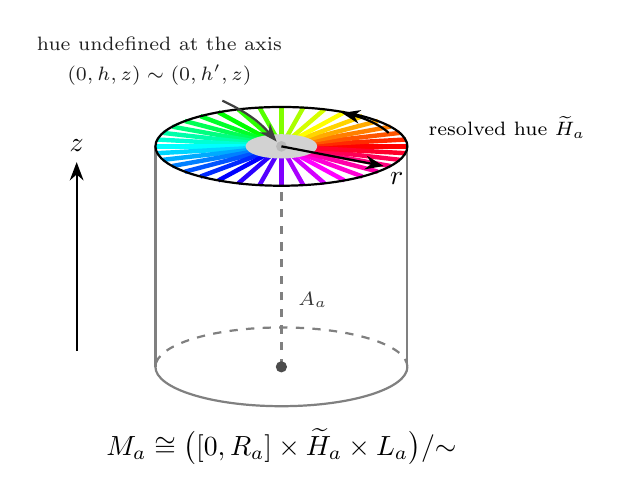
\begin{tikzpicture}[>=Stealth, line width=0.8pt]

  \draw[dashed, gray] (1.6,-1.4) arc[start angle=0, end angle=180,
    x radius=1.6, y radius=0.5];
  \draw[gray] (1.6,-1.4) arc[start angle=0, end angle=-180,
    x radius=1.6, y radius=0.5];
  \draw[gray] (-1.6,-1.4) -- (-1.6,1.4);
  \draw[gray] ( 1.6,-1.4) -- ( 1.6,1.4);
  \draw[gray, dashed] (0,-1.4) -- (0,1.4);
  \filldraw[gray!60!black] (0,-1.4) circle (1.6pt);

  \foreach \k in {0,...,35}{
    \pgfmathsetmacro{\hue}{\k/36}
    \pgfmathsetmacro{\ang}{\k*10}
    \definecolor{spokecol}{hsb}{\hue,1,1}
    \draw[spokecol, line width=1.6pt]
      (0,1.4) -- ({1.6*cos(\ang)},{1.4+0.5*sin(\ang)});
  }
  \filldraw[gray!35] (0,1.4) ellipse[x radius=0.44, y radius=0.14];
  \filldraw[gray!55!white] (0,1.4) circle (1.5pt);
  \draw (0,1.4) ellipse[x radius=1.6, y radius=0.5];

  \draw[->] (-2.6,-1.2) -- (-2.6,1.2);
  \node[above] at (-2.6,1.2) {$z$};
  \draw[->, black] (0,1.4) -- ({1.5*cos(-30)},{1.4+0.5*sin(-30)});
  \node[below right=-2pt] at ({1.5*cos(-30)},{1.4+0.5*sin(-30)}) {$r$};
  \draw[->, black] ({1.45*cos(20)},{1.4+0.5*sin(20)})
    arc[start angle=20, end angle=58, x radius=1.45, y radius=0.5];
  \node[right] at (1.74,1.64) {\scriptsize resolved hue $\widetilde H_a$};
  \node[right=1pt, gray!40!black] at (0.05,-0.55) {\scriptsize $A_a$};

  \draw[->, gray!50!black] (-0.75,1.98) to[bend left=12] (-0.06,1.46);
  \node[anchor=south, align=center, gray!25!black] at (-1.55,2.04)
    {\scriptsize hue undefined at the axis\\[-1pt]
     \scriptsize $(0,h,z)\sim(0,h',z)$};

  \node[anchor=north] at (0,-2.05)
    {$M_a\cong\bigl([0,R_a]\times\widetilde H_a\times L_a\bigr)/{\sim}$};

\end{tikzpicture}
\caption{The vivid color body $M_a$ and its achromatic quotient.
Saturation $r$ is radial, resolved hue $\widetilde H_a$ angular, and
luminosity $z$ vertical. At zero saturation, hue is undefined: all hue
labels are identified along the achromatic axis $A_a=\{r=0\}$ via
$(0,h,z)\sim(0,h',z)$, so the hue wheel washes out to neutral gray at
the center. The ambient color body $M_a$ is the full cylinder; the
narrowing to a stimulus-reachable spindle is the separate reachability
constraint introduced in \Cref{sec:reachability}.}
\label{fig:color-body}
\end{figure}

\subsection{The chromatic stratum}
\label{subsec:chromatic-stratum}

\noindent Let
\[
A_a=\{r=0\}\subset M_a
\]
denote the achromatic axis, and define the chromatic stratum
\[
M_a^{\ast}=M_a\setminus A_a.
\]
On $M_a^{\ast}$, saturation is nonzero and the hue coordinate is well-defined. Choosing the angular coordinate
\[
\theta:\widetilde H_a\longrightarrow\mathbb{R}/2\pi\mathbb{Z}
\]
calibrated in \Cref{sec:compactification}, the chromatic stratum admits local coordinates $(r,\theta,z)$.

This is the only domain on which it is mathematically correct to regard the color body as a bundle over hue. On $M_a^{\ast}$ there is a smooth projection
\[
M_a^{\ast}\longrightarrow\widetilde H_a,
\]
with local fiber coordinates $(r,z)$. At $r=0$, this projection ceases to be defined because all hue values have been quotiented to a single point. The global color body is therefore not a fiber bundle over the hue circle; only its chromatic stratum is.

This distinction prevents a common formal error. A cylindrical coordinate system is appropriate for chromatic color, but it should not be mistaken for a global product structure on the full color body. The achromatic axis is not an additional hue. It is the geometric locus at which hue disappears.

\subsection{The local indefinite metric}
\label{subsec:local-indefinite-metric}

\noindent On the chromatic stratum $M_a^{\ast}$ (where the asterisk denotes the restriction away from the achromatic axis $r=0$ to bypass the standard polar coordinate singularity), we introduce the idealized flat normal form of the local metric:
\[
g_a=dr^{2}+r^{2}d\theta^{2}-\kappa_a^{2}dz^{2},
\]
where $\kappa_a>0$ is a constant scalar fixing the relative scale between chromatic displacement and luminosity displacement for an isotropic visual regime $a$.

The positive term $dr^{2}+r^{2}d\theta^{2}$ is the ordinary polar metric on the chromatic plane, measuring displacement in saturation and hue. The negative term $-\kappa_a^{2}dz^{2}$ assigns the luminosity coordinate the opposite metric sign.

The angular component of this baseline metric is the bare polar term $r^2\,d\theta^2$. This is a deliberate choice of normal form, not a claim that perceptual hue discrimination is isotropic with coordinate angle: it is the flat reference geometry against which empirical anisotropy is later measured. When the model is calibrated in \Cref{sec:reachability}, the angular component is promoted to a hue- and saturation-dependent field that reduces to $r^2$ near the achromatic axis but carries the empirical discrimination geometry near the boundary. The bare $r^2$ here should therefore be read as the $r\to 0$ limit of that field, deferred to \Cref{sec:reachability} for its calibrated form.

It is necessary to explicitly distinguish this geometry from classical mathematical colorimetry. There is a century-long tradition of applying differential geometry to color space, codified by \citet{Schrodinger1920} and formalized through the MacAdam ellipses \citep{MacAdam1942} and Resnikoff's symmetric geometries \citep{Resnikoff1974}. In these classical models, the metric is strictly positive-definite --- signature $(3,0)$ --- and the metric tensor $ds^2$ represents Just-Noticeable Differences (JNDs), mapping the static subjective discrimination distance between two adjacent colors.

Recent empirical work has further challenged the Riemannian paradigm itself: \citeauthor{Bujack2022} demonstrate that large color differences are perceived as less than the sum of small steps --- a diminishing-returns effect incompatible with any Riemannian metric construed as a global model of perceived color difference \citep{Bujack2022}. The result constrains the \emph{composition} of a perceptual distance functional along paths: it shows that the geodesic distance between two colors cannot be recovered by integrating local discriminability, since large differences fall short of the summed small ones. Crucially, this is a statement about a path-integrated, positive-definite \emph{distance}, not about the local tangent structure at a point; Bujack et al.\ explicitly do not exclude loci that are locally Riemannian.

The kinematic $(2,1)$ metric introduced here is not directly targeted by this objection, and the immunity is structural rather than terminological. The indefinite metric is not invoked as a perceptual distance functional at all. Its role is to supply a \emph{conformal causal structure} --- the field of null cones partitioning each tangent space into chromatic-spacelike and luminosity-timelike directions --- which bounds the reachability body of \Cref{sec:reachability}. A conformal causal structure and a Riemannian distance functional are different objects: the former is invariant under $g\mapsto\Omega^2 g$ and assigns no path length, while the latter has no null cone at all. Bujack's result falsifies the second as a model of color difference; it does not directly constrain the first. Concretely, moving along a null vector ($ds^2=0$) does not assert zero perceptual difference between a maximally dark and a saturated color --- which would be empirically absurd --- because the metric does not measure perceptual difference; it measures reachability. The $(2,1)$ metric is in this sense a \emph{kinematic gauge}, not a discriminability metric. It models the dynamic control space, causal horizons, and physiological zero-sum tradeoffs (exhaustion limits) of the visual network.

The indefinite signature is therefore introduced here as a local normal form to govern dynamic state transitions, not derived from topology or static discriminability alone. Its justification is deferred to \Cref{sec:reachability}, where the Lorentzian causal structure of this pseudo-Riemannian metric is used to model the kinematic boundary between ordinary continuous optical inputs and discrete physiological shifts (chimerical colors). The purpose of the minus sign is not merely to distinguish luminosity from hue; rather, once the scale $\kappa_a$ is fixed, it calibrates the geometry such that the physiological exhaustion limits of the visual network coincide with the null hypersurfaces of the (scale-free) causal structure, establishing a mathematically rigorous reachability horizon in phenomenal color space.

The metric has signature $(2,1)$ on the chromatic stratum. The scalar parameter $\kappa_a$ is not merely notational. In the present section it establishes the idealized baseline scale; in \Cref{sec:reachability} it determines the absolute slope of the idealized optical reachability envelope.

\subsection{Split-complex radial--luminosity sections}
\label{subsec:split-complex-sections}

\noindent For each fixed hue angle $\theta$, define the radial--luminosity section
\[
\Sigma_{\theta}=\{(r,\theta,z)\in M_a^{\ast}: r>0,\ z\in L_a\}.
\]
Since saturation is non-negative, $\Sigma_{\theta}$ is a half-plane in the radial--luminosity variables rather than the full plane. In the uncurved normal form, the induced quadratic form has a constant split signature:
\[
g_{\theta}=dr^{2}-\kappa_a^{2}dz^{2}.
\]
Thus each fixed-hue radial--luminosity section carries a split-complex metric of signature $(1,1)$.

Equivalently, introduce a local split-complex coordinate
\[
q_{\theta}=r+j\kappa_a z,
\qquad
j^{2}=+1.
\]
With split-complex conjugation $\overline q_{\theta}=r-j\kappa_a z$, the associated split norm is
\[
N(q_{\theta})=q_{\theta}\overline q_{\theta}=r^{2}-\kappa_a^{2}z^{2}.
\]
This is exactly the quadratic form induced by the flat baseline metric $g_{\theta}$. The state-space section uses the half-plane $r>0$, but the local quadratic form maps to the standard split-complex form.

The algebraic transition to a split-complex half-plane is not a mere notational convenience; it dictates the permissible symmetry transformations within the fixed-hue section. In standard complex geometry, phase multiplication generates Euclidean rotations. In the split-complex geometry, multiplication by a split-phase factor $e^{j\phi}$ generates a hyperbolic rotation (a Lorentz boost) that mixes the radial saturation coordinate with the luminosity coordinate. This is the algebraic counterpart of a known perceptual phenomenon: the Hunt effect, in which higher luminance systematically raises the perceived colorfulness (chroma) of a stimulus \citep{Hunt1952,Fairchild2013}. The split-complex structure makes a specific structural prediction about this effect --- that to first order it acts as a hyperbolic rotation in the radial--luminosity plane, preserving the split norm $r^2-\kappa_a^2 z^2$ --- which a fully calibrated adaptation model could test. We do not pursue that calibration here; the point is that the algebra of the fixed-hue section is not inert, but carries a falsifiable commitment about the form of luminance-induced changes in perceived saturation. Hue shifts with intensity, by contrast --- the Bezold--Brücke effect --- are \emph{not} captured by this operation: $e^{j\phi}$ acts on $q_\theta$ alone and holds the section label $\theta$ fixed, so an intensity-dependent hue shift would require a mechanism coupling distinct fixed-hue sections, which the split-complex normal form does not supply \citep{Purdy1931}.

It should be noted that this algebraic rigidity strictly applies to the idealized flat normal form. When biological bounds introduce internal curvature to the metric (as developed in \Cref{sec:reachability}), these sections generalize to curved pseudo-Riemannian 2-manifolds, though the local tangent space $T_p\Sigma_\theta$ preserves the exact split-complex algebraic structure.

The hue coordinate labels the section; it is not an additional component of the split-complex number. The model does not identify a color state with a global algebraic object of the form ``complex hue plus split luminosity.'' Such a construction would introduce an additional real degree of freedom and overdetermine the phenomenology. Instead, the full color body remains three-dimensional, while each fixed-hue radial--luminosity section locally supports a split-complex structure: an $S^1$-family of split-complex two-planes, not a single global four-dimensional algebra.

\subsection{The achromatic axis and tensor hygiene}
\label{subsec:achromatic-axis}

\noindent The flat baseline expression
\[
g_a=dr^{2}+r^{2}d\theta^{2}-\kappa_a^{2}dz^{2}
\]
is written in cylindrical chromatic coordinates. These coordinates fail at $r=0$ because the phase angle $\theta$ is undefined there. This coordinate failure corresponds exactly to the achromatic axis $A_a$: at absolute zero saturation, there is luminosity but no chromatic phase.

The metric tensor itself does not degenerate at the achromatic axis. To see this, introduce Cartesian chromatic coordinates
\[
x=r\cos\theta,\qquad y=r\sin\theta.
\]
Because the total affine length of the resolved hue circle was calibrated to exactly $2\pi$ in \Cref{sec:compactification}, this coordinate transformation is a valid diffeomorphism on the punctured chromatic plane, and the polar coordinate singularity resolves smoothly without leaving a conical deficit. Since $\kappa_a$ is a constant in this idealized normal form, the luminosity term $-\kappa_a^2 dz^2$ contains no angular dependence, and the local metric transforms to:
\[
g_a=dx^{2}+dy^{2}-\kappa_a^{2}dz^{2}.
\]
This expression is exact and nondegenerate at $x=y=0$. What fails at the achromatic axis is not the metric, but the polar hue coordinate. The cylindrical chart therefore does not contain the achromatic axis as coordinate points: with $\theta$ undefined at $r=0$, each neutral state is realized only as the limit of chromatic states along an $r\to 0$ ray, and is recovered as a genuine point solely in the Cartesian chart. The neutral locus is in this sense ``approach-only'': there is no single neutral state bearing a chromatic phase.

The geometry thus matches the phenomenology: gray is not a metrically singular or degenerate color state; it is simply a well-defined state in which chromatic phase is absent. This establishes a strict constraint for the ensuing sections: any biologically induced curvature added to the manifold (such as promoting the constant scale factor $\kappa_a$ to a hue-dependent scalar field $\kappa(\theta)$ to model anisotropic empirical gamuts) must decay to this regular, $\theta$-independent Cartesian form as $r\to 0$. Failure to enforce this decay would produce a multi-valued metric tensor at the achromatic axis, shattering the quotient space.

This clarifies exactly why the topological quotient definition of $M_a$ is necessary. Without the identification $(0,h,z)\sim(0,h',z)$, one would artificially multiply gray states by all possible hues. The quotient removes these spurious hue labels and leaves a single smooth achromatic axis parameterized strictly by luminosity.

\subsection{Scope of the metric model}
\label{subsec:metric-model-scope}

\noindent The metric model introduced here is a structural normal form. It isolates the local distinction between chromatic rotation, radial saturation, and luminosity polarity, while leaving open the empirical calibration of the accessible color body. Actual empirical color bodies may be anisotropic, observer-dependent, or deformed by the nonlinear biological constraints of the visual regime. Those empirical complications will alter the scale factor and induce internal curvature. They do not, however, remove the formal distinction between cyclic hue, radial saturation, and achromatic luminosity.

The central claim of this section is therefore limited but exact. The vivid color body $M_a$ is a real three-dimensional pseudo-Riemannian phenomenal manifold. Its chromatic stratum admits local coordinates $(r,\theta,z)$ carrying an indefinite metric of signature $(2,1)$, whose causal reachability interpretation is developed in \Cref{sec:reachability}. At each fixed hue, the tangent space to the radial--luminosity section carries a split-complex quadratic form of signature $(1,1)$.

No reachability boundary has yet been introduced. The present section supplies the local indefinite metric structure needed to define one. \Cref{sec:reachability} uses this geometry to mathematically formalize the color spindle as a kinematic reachability body, separating ordinary stimulus-accessible colors from the spacelike exterior of chimerical colors.

%%%%%%%%%%%%%%%%%%%%%%%%%%%%%%%%%%%%%%%%%%%%%%%%%%%%%%%%%%%%%%%%%%%%%%%%%%
%%% SECTION 5: THE COLOR SPINDLE AS REACHABILITY BODY
%%%%%%%%%%%%%%%%%%%%%%%%%%%%%%%%%%%%%%%%%%%%%%%%%%%%%%%%%%%%%%%%%%%%%%%%%%
\section{The Color Spindle as Reachability Body}
\label{sec:reachability}

Section~\ref{sec:local-model} introduced an indefinite local metric on the vivid color body $M_a$, while deliberately postponing its reachability interpretation. The present section supplies that interpretation. The indefinite metric is not claimed to follow from topology alone, nor merely from the fact that luminosity is different from hue. Its role is to provide a calibrated normal form for representing the kinematic boundary between ordinary stimulus-accessible colors and chimerical colors.

A point of method should be stated at the outset, because it governs how every claim in this section is to be read. The metric introduced below is not derived from an independent dynamical principle and then found to bound the empirical gamut. It is the reverse: the macroscopic slopes of the empirically observed color solid are taken as given, and the metric is constructed---reverse-engineered---so that those slopes are its null hypersurfaces. The content of the model therefore does not lie in predicting the gross bicone shape, which is an input. It lies in what the null-boundary requirement then forces: a $C^0$ equatorial ridge as a structural necessity rather than an artifact (\Cref{subsec:idealized-flat-normal-form}), and a coordinate-invariant admissibility bound relating the hue-dependent saturation ceiling to the local discrimination geometry (\Cref{subsec:eikonal-constraint}). These consequences are not built in; they are what the construction yields once the bicone is taken as the boundary. We flag the reverse-engineering explicitly so that the falsifiable content is not mistaken for the calibration.

The color spindle \citep{Churchland2005} provides the relevant empirical structure. Ordinary colors occupy the familiar stimulus-accessible region of color experience. Chimerical or impossible colors are phenomenally possible, and may be induced under altered physiological conditions, but they lie outside the ordinary range accessible by continuous optical stimulation under normal operating conditions. The present section formalizes this distinction by treating the spindle as a kinematic reachability body inside $M_a$. \Cref{fig:spindle} depicts the symmetric reachability normal form and its
piecewise null boundary.

\begin{figure}[t]
\centering
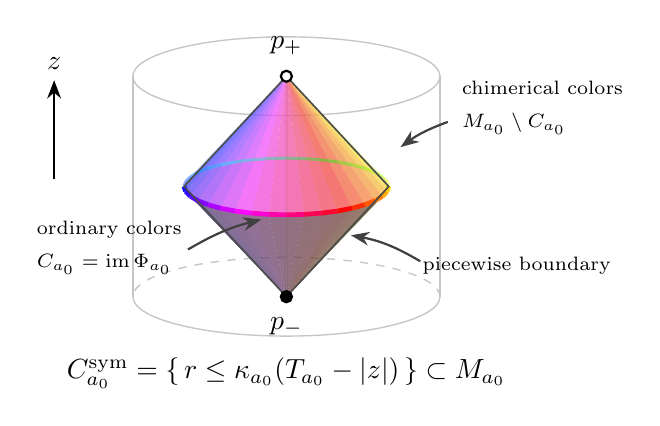
\begin{tikzpicture}[>=Stealth, line width=0.8pt]

  \draw[gray!45,dashed,line width=0.5pt] (1.95,-1.4) arc[start angle=0,end angle=180,x radius=1.95,y radius=0.5];
  \draw[gray!45,line width=0.5pt]         (1.95,-1.4) arc[start angle=0,end angle=-180,x radius=1.95,y radius=0.5];
  \draw[gray!45,line width=0.5pt] (-1.95,-1.4)--(-1.95,1.4);
  \draw[gray!45,line width=0.5pt] ( 1.95,-1.4)--( 1.95,1.4);
  \draw[gray!45,line width=0.5pt] (0,1.4) ellipse[x radius=1.95,y radius=0.5];

  \foreach \i in {0,...,17}{
    \pgfmathsetmacro{\pa}{\i*10}\pgfmathsetmacro{\pb}{(\i+1)*10}
    \pgfmathsetmacro{\hueval}{mod(\i/36+0.16667,1)}
    \definecolor{hh}{hsb}{\hueval,1,1}
    \pgfmathsetmacro{\xa}{1.3*cos(\pa)}\pgfmathsetmacro{\ya}{0.36*sin(\pa)}
    \pgfmathsetmacro{\xb}{1.3*cos(\pb)}\pgfmathsetmacro{\yb}{0.36*sin(\pb)}
    \fill[hh!52!black,fill opacity=0.18] (\xa,\ya)--(\xb,\yb)--(0,-1.4)--cycle;
    \fill[hh!78!white,fill opacity=0.18] (\xa,\ya)--(\xb,\yb)--(0, 1.4)--cycle;
  }

  \draw[gray!60,line width=1pt,opacity=0.55] (0,-1.32)--(0,1.32);

  \foreach \i in {18,...,35}{
    \pgfmathsetmacro{\pa}{\i*10}\pgfmathsetmacro{\pb}{(\i+1)*10}
    \pgfmathsetmacro{\hueval}{mod(\i/36+0.16667,1)}
    \definecolor{hh}{hsb}{\hueval,1,1}
    \pgfmathsetmacro{\xa}{1.3*cos(\pa)}\pgfmathsetmacro{\ya}{0.36*sin(\pa)}
    \pgfmathsetmacro{\xb}{1.3*cos(\pb)}\pgfmathsetmacro{\yb}{0.36*sin(\pb)}
    \fill[hh!45!black,fill opacity=0.70] (\xa,\ya)--(\xb,\yb)--(0,-1.4)--cycle;
    \fill[hh!72!white,fill opacity=0.70] (\xa,\ya)--(\xb,\yb)--(0, 1.4)--cycle;
  }

  \foreach \i in {0,...,17}{
    \pgfmathsetmacro{\pa}{\i*10}\pgfmathsetmacro{\pb}{(\i+1)*10}
    \pgfmathsetmacro{\hueval}{mod(\i/36+0.16667,1)}\definecolor{hh}{hsb}{\hueval,1,1}
    \draw[hh,line width=1.1pt,opacity=0.40]
      ({1.3*cos(\pa)},{0.36*sin(\pa)})--({1.3*cos(\pb)},{0.36*sin(\pb)});
  }
  \foreach \i in {18,...,35}{
    \pgfmathsetmacro{\pa}{\i*10}\pgfmathsetmacro{\pb}{(\i+1)*10}
    \pgfmathsetmacro{\hueval}{mod(\i/36+0.16667,1)}\definecolor{hh}{hsb}{\hueval,1,1}
    \draw[hh,line width=1.7pt,opacity=0.95]
      ({1.3*cos(\pa)},{0.36*sin(\pa)})--({1.3*cos(\pb)},{0.36*sin(\pb)});
  }

  \draw[black!70,line width=0.6pt]
    (0,-1.4)--(1.3,0)--(0,1.4)--(-1.3,0)--cycle;

  \filldraw[draw=black,fill=white] (0, 1.4) circle (2pt);
  \filldraw[draw=black,fill=black] (0,-1.4) circle (2pt);
  \node[above=1pt] at (0,1.5){$p_+$};
  \node[below=1pt] at (0,-1.5){$p_-$};

  \draw[->] (-2.95,0.1)--(-2.95,1.35);
  \node[above] at (-2.95,1.35){$z$};

  \node[anchor=west,align=left] at (-3.3,-0.78)
    {\scriptsize ordinary colors\\ \scriptsize $C_{a_0}=\operatorname{im}\Phi_{a_0}$};
  \draw[->,gray!50!black] (-1.25,-0.8) to[bend left=8] (-0.32,-0.42);
  \node[anchor=west,align=left] at (2.1,1.0)
    {\scriptsize chimerical colors\\ \scriptsize $M_{a_0}\setminus C_{a_0}$};
  \draw[->,gray!50!black] (2.05,0.82) to[bend right=8] (1.45,0.5);
  \node[anchor=west] at (1.6,-1.0){\scriptsize piecewise boundary};
  \draw[->,gray!50!black] (1.7,-0.95) to[bend right=10] (0.82,-0.62);

  \node[anchor=north] at (0,-2.05)
    {$C_{a_0}^{\mathrm{sym}}=\{\,r\le\kappa_{a_0}(T_{a_0}-|z|)\,\}
    \subset M_{a_0}$};

\end{tikzpicture}
\caption{The color spindle as a calibrated reachability body inside the
ambient vivid color body $M_{a_0}$. Hue runs around the equator at full
saturation; tints lighten toward the white pole $p_+$, shades darken
toward the black pole $p_-$, and saturation falls to the neutral
achromatic axis $A_{a_0}$ at the gray core. The ordinary optical image
$C_{a_0}=\operatorname{im}\Phi_{a_0}$ is represented in symmetric normal
form by the $C^0$ bicone
$C_{a_0}^{\mathrm{sym}}=\{\,r\le\kappa_{a_0}(T_{a_0}-|z|)\,\}$.
Empirical calibration may deform this idealized body. The geometric
distinction, however, remains structurally consistent: the boundary is
modeled locally as a piecewise null hypersurface (forming a ridge at the
equator), while the exterior $M_{a_0}\setminus C_{a_0}$ represents
chimerical states accessible only after alteration of the visual operating
regime \citep{Churchland2005}.}
\label{fig:spindle}
\end{figure}

The key claim is not that every ordinary color transition is timelike. That would be false: ordinary isoluminant hue shifts may have spacelike tangent vectors with respect to the local metric. The claim is narrower. The boundary is a calibrated geometric representation of the extremal kinematic envelope of ordinary optical reachability: the formal limit surface beyond which continuous optical stimulation, under a fixed operating regime, is dynamically restricted from crossing.

\subsection{The ordinary optical image and the Hurvich--Jameson coordinate mapping}
\label{subsec:ordinary-optical-image}

Let $a_0$ denote a fixed ordinary visual operating regime for the observer. Let
\[
\Phi_{a_0}:\mathcal{S}_{\mathrm{ord}}^{a_0}\longrightarrow M_{a_0}
\]
be the perceptual response map from ordinary spectral power distributions, under the fixed operating regime $a_0$, into the vivid phenomenal color body $M_{a_0}$. The ordinary color spindle is the image
\[
C_{a_0}=\operatorname{im}(\Phi_{a_0})\subset M_{a_0}.
\]
Thus $C_{a_0}$ is not the full space of phenomenally possible color appearances. It is the restricted region accessible by ordinary continuous optical stimulation while the visual system remains in its normal operating state.

To ground this abstract geometry in established neurobiology, we explicitly map the coordinates of $M_{a_0}$ to the Hurvich--Jameson opponent-cell activation outputs formalized by \citet{Churchland2005}. In this network, color is represented in a three-dimensional activation space driven by Green/Red ($A_{G/R}$), Blue/Yellow ($A_{B/Y}$), and White/Black ($A_{W/B}$) opponent cells, each with a resting baseline of 50\% activation. Following Churchland's equations $A_{G/R}=50+(L-M)/2$ and $A_{B/Y}=50+(L+M)/4-S/2$, the Green/Red cell rises above baseline for red-dominant stimuli and falls below for green-dominant stimuli, while the Blue/Yellow cell rises above baseline for yellow-dominant stimuli and falls below for blue-dominant stimuli. We translate the resting baseline to the geometric coordinate singularity $(0,0,0)$ and define the Cartesian chromatic coordinates as signed excursions from it:
\[
x = A_{G/R} - 50,\qquad y = A_{B/Y} - 50,\qquad z = A_{W/B} - 50,
\]
so that $x>0$ encodes red dominance, $x<0$ green dominance, $y>0$ yellow dominance, and $y<0$ blue dominance.

The cylindrical chromatic coordinates $(r,\theta,z)$ then emerge directly from the biological outputs:
\[
r = \sqrt{(A_{G/R}-50)^2+(A_{B/Y}-50)^2},\qquad
\theta = \operatorname{atan2}(A_{B/Y}-50,\,A_{G/R}-50).
\]
The opponent-channel architecture supplies a physiological realization of the response-side hue coordinate used in the compactification and resolution model of \Cref{sec:compactification}. In particular, the line of purples is represented as a one-dimensional response-side arc within the sector jointly expressing red-side and blue-side opponent activation, i.e. the sector with $x>0$ and $y<0$ in the present Hurvich--Jameson coordinates. This sector should not be identified with the exceptional fiber itself: the quadrant is a two-dimensional region of the chromatic plane, while $P_a$ is a one-dimensional family of hue directions. Nor is it necessary to claim that the entire quadrant lacks a monochromatic preimage. The nonspectral claim applies to the purple arc/fiber. Its points are nonspectral in the sense of \Cref{sec:magenta-gap}: their metameric classes do not intersect the idealized monochromatic locus. Operationally, they are induced paradigmatically by spectral measures with joint short- and long-wavelength contributions rather than by a single Dirac stimulus $\sigma_\lambda$. Thus the purple arc through this opponent sector furnishes the smooth phase coordinate $\theta$ that closes the hue circle without adding any new physical wavelength.

The $r=0$ coordinate singularity introduced in \Cref{sec:local-model} is not a mathematical artifact. It is the exact physiological state where both the Green/Red and Blue/Yellow opponent cells sit at their neutral baselines --- a state completely devoid of chromatic phase. The black pole $p_-=(0,0,-T_{a_0})$ does not represent this neutral origin but rather the maximal negative excursion of the White/Black channel, driven by a focal region dark against a brighter surround. Because $A_{W/B}$ assays focal intensity relative to the surround rather than absolute incident power, the luminosity axis is intrinsically relational: its poles $p_\pm$ are extremes of focal-versus-surround contrast, not of absolute light level.

\subsection{The idealized flat normal form}
\label{subsec:idealized-flat-normal-form}

Before introducing empirical deformations, we establish the baseline geometry of the ordinary optical image in an idealized, perfectly symmetric state. As introduced in \Cref{sec:local-model}, we assign the chromatic stratum a flat pseudo-Riemannian metric:
\[
g_{a_0}=dx^{2}+dy^{2}-\kappa_{a_0}^{2}dz^{2},
\]
where $\kappa_{a_0}>0$ is a constant scale factor relating chromatic displacement to luminosity displacement.

Assume the luminosity interval is centered and bounded, $L_{a_0}=[-T_{a_0},T_{a_0}]$, with $T_{a_0}>0$. The two achromatic limiting poles are $p_-=(0,0,-T_{a_0})$ and $p_+=(0,0,T_{a_0})$. Define the quadratic forms corresponding to the squared intervals from the lower and upper achromatic poles:
\[
Q_-(x,y,z)=x^{2}+y^{2}-\kappa_{a_0}^{2}(z+T_{a_0})^{2},
\]
\[
Q_+(x,y,z)=x^{2}+y^{2}-\kappa_{a_0}^{2}(T_{a_0}-z)^{2}.
\]
The symmetric reachability body is defined as the intersection of the future of the lower achromatic pole and the past of the upper achromatic pole --- a structure geometrically identical to an Alexandrov interval (causal diamond):
\[
C_{a_0}^{\mathrm{sym}}
=\{Q_-\leq 0\}\cap\{Q_+\leq 0\}\cap\{-T_{a_0}\leq z\leq T_{a_0}\}.
\]
Equivalently, the maximal chromatic radius collapses linearly toward the achromatic poles: $r\leq\kappa_{a_0}(T_{a_0}-|z|)$.

To see geometrically why this boundary constitutes a formal limit of phenomenal access, parameterize the lower boundary surface by $s\in[0,T_{a_0}]$, starting from the black pole $p_-$ at $s=0$ and reaching the equator at $s=T_{a_0}$:
\[
\gamma_-^{\theta}(s)=
\bigl(\kappa_{a_0}s\cos\theta,\;\kappa_{a_0}s\sin\theta,\;
-T_{a_0}+s\bigr).
\]
The tangent vector is $\dot\gamma_-^{\theta}=(\kappa_{a_0}\cos\theta,\;\kappa_{a_0}\sin\theta,\;1)$, and its norm in the flat metric $g_{a_0}$ evaluates to:
\[
g_{a_0}(\dot\gamma_-^{\theta},\dot\gamma_-^{\theta})
=\kappa_{a_0}^2\cos^2\theta+\kappa_{a_0}^2\sin^2\theta-\kappa_{a_0}^2
=\kappa_{a_0}^2-\kappa_{a_0}^2=0.
\]
The identical cancellation holds for the upper boundary paths from $p_+$. The boundary generators are strictly \emph{null} curves. As stated at the outset of this section, defining the boundary as a null hypersurface ($ds^2=0$) is the reverse-engineering step: the metric scale is fixed so that the macroscopic slopes of the empirical bicone are null. What the null generators then encode is that the magnitude of chromatic displacement exactly equals the luminosity displacement along the boundary --- the geometric signature of opponent-channel exhaustion at the kinematic horizon of the visual system.

The bicone features a non-differentiable $C^0$ ridge at the equator ($z=0$) where the two null cones intersect. This ridge is not an incidental feature of the symmetric idealization; it is forced. Proposition~\ref{prop:no-smooth-null} below establishes that a compact reachability body with a smooth (everywhere-differentiable) null boundary cannot exist in a signature-$(2,1)$ manifold, so any null reachability envelope closing across an isoluminant equator must do so along a non-differentiable ridge. This is the structural prediction previewed in \Cref{sec:introduction}: the equatorial ridge of an empirical color solid is, under this model, a necessary geometric feature rather than measurement noise to be smoothed away.

\subsection{Biological realism: the hue-dependent saturation ceiling}
\label{subsec:biological-realism-squashing-function}

The symmetric bicone generated by a constant $\kappa_{a_0}$ serves only as an idealized baseline. In biological reality, the empirical maximum saturation of human vision varies significantly by hue; the visual system's capacity to reach saturated yellow differs structurally from its capacity for saturated blue.

We encode this hue dependence by upgrading the constant scale factor $\kappa_{a_0}$ to a hue-dependent smooth scalar field $\alpha(\theta)$. The symbols are deliberately distinct: $\kappa_{a_0}$ is the isotropic scale of the symmetric idealization, whereas $\alpha(\theta)$ is the anisotropic, empirically calibrated saturation ceiling. The deformed empirical reachability boundary is:
\[
R_{a_0}(\theta,z)=\alpha(\theta)(T_{a_0}-|z|).
\]
Superimposing this boundary over the globally flat metric $g_{a_0}$ breaks the null condition just established. If the empirical boundary is to remain a modeled kinematic null horizon --- the foundational requirement of this calibrated model --- the metric itself cannot remain flat. The phenomenal manifold must acquire internal curvature induced by the visual system's specific biological calibration. This curvature must be managed carefully to ensure the interior chromatic stratum remains $C^\infty$ while preserving the $C^0$ nature of the equatorial intersection. The next subsection shows that the requirement of a null boundary bounding a regular interior is not automatically satisfiable, and that its satisfiability is governed by a single coordinate-invariant inequality.

\subsection{A Coordinate-Invariant Gamut Bound}
\label{subsec:eikonal-constraint}

\noindent The deformed empirical boundary
\[
R_{a_0}(\theta,z)=\alpha(\theta)(T_{a_0}-|z|)
\]
must meet two requirements at once. It must be a \emph{null} hypersurface of the metric, so that it functions as a reachability horizon; and the region it bounds must remain a genuine signature-$(2,1)$ interior, with positive-definite spatial block and no coordinate singularity short of the boundary itself. These two demands are not automatically compatible. We show that their compatibility is controlled by a single coordinate-invariant inequality, and that this inequality is not an extra stipulation but is exactly the condition that the radial metric component remain positive in the interior.

In the general unrotated coordinate frame, the spatial metric includes a generic cross-term $D(r,\theta,z)$ between the radial and angular components:
\[
ds^2
=
A(r,\theta,z)\,dr^2
+2D(r,\theta,z)\,dr\,d\theta
+B(r,\theta,z)\,d\theta^2
-C(r,\theta,z)\,dz^2 .
\]
The spatial block $\begin{psmallmatrix} A & D\\ D & B\end{psmallmatrix}$ has determinant $\Delta=AB-D^2$, positive precisely when the spatial metric is positive-definite.

We first establish that the boundary cannot be smooth, which forces the piecewise structure used throughout.

\begin{proposition}[No smooth null envelope]
\label{prop:no-smooth-null}
Let $g$ be a metric of signature $(2,1)$ on the chromatic stratum with positive-definite spatial block, and let $C$ be a compact reachability body whose boundary $\partial C$ is a null hypersurface of $g$. Then $\partial C$ is not everywhere differentiable. In the symmetric normal form, the non-differentiable locus is the isoluminant equatorial ridge.
\end{proposition}

\begin{proof}
Write the boundary locally as $r=R(\theta,z)$ with implicit function $F=r-R$ and normal covector $n_\mu=\partial_\mu F=(1,-R_\theta,-R_z)$. By compactness, the chromatic radius $r$ attains a maximum along the boundary at fixed $\theta$; at such a point $\partial_z R=0$, so $R_z=0$ and the normal covector is purely spatial, $n_\mu=(1,-R_\theta,0)$. The null condition $g^{\mu\nu}n_\mu n_\nu=0$ then reduces to its spatial part $g^{ij}n_i n_j=0$, since the luminosity contribution $g^{zz}n_z^2$ vanishes. But the spatial block is positive-definite, hence so is its inverse, and $n_i=(1,-R_\theta)\neq 0$ because $n_r=1$. Therefore $g^{ij}n_i n_j>0$ strictly, contradicting the null condition. No point with $\partial_z R=0$ can lie on a smooth null boundary; since compactness forces such a point to exist, $\partial C$ cannot be smooth there.
\end{proof}

Accordingly we define $\partial C_{a_0}$ as the piecewise union of two smooth null hypersurfaces meeting along the equatorial ridge,
\[
\partial C_{a_0}=\Sigma_+\cup\Sigma_-,
\qquad
\Sigma_+=\{r=\alpha(\theta)(T_{a_0}-z)\mid z\geq 0\},
\quad
\Sigma_-=\{r=\alpha(\theta)(T_{a_0}+z)\mid z\leq 0\},
\]
with implicit boundary function $F(r,\theta,z)=r-R_{a_0}(\theta,z)$: the interior is $F\leq 0$, the exterior $F>0$. The null condition is imposed on each open piece $z>0$ and $z<0$ separately.

\paragraph{The null condition}
For the normal covector $n_\mu=(1,-R_\theta,-R_z)$ the null condition $g^{\mu\nu}\partial_\mu F\,\partial_\nu F=0$ evaluates to
\[
\frac{B(1)^2-2D(-R_\theta)(1)+A(-R_\theta)^2}{\Delta}
-\frac{1}{C}(R_z)^2=0.
\]
On $\Sigma_+$, where $R_{a_0}=\alpha(\theta)(T_{a_0}-z)$,
\[
R_\theta=\alpha'(\theta)(T_{a_0}-z),
\qquad
R_z=-\alpha(\theta).
\]
We define $\alpha(\theta)$ geometrically as the value of $\sqrt{C}$ at the boundary, $C|_{\partial C_{a_0}}=\alpha(\theta)^2$, so that the luminosity contribution is normalized:
\[
\frac{R_z^2}{C}=\frac{\alpha(\theta)^2}{\alpha(\theta)^2}=1.
\]
Multiplying through by $\Delta$ gives
\[
B+2D\,R_\theta+A\,R_\theta^2
=
\Delta
=
AB-D^2.
\tag{$*$}
\]
The identical relation holds on $\Sigma_-$: the sign of $R_z$ reverses but $R_z^2/C$ is unchanged.

\paragraph{Gauge-independence of the bound}
To verify that the resulting constraint is independent of the radial--angular gauge and absorbs the cross-term $D$, multiply $(*)$ by $B$ and subtract $R_\theta^2(AB-D^2)$ from both sides:
\[
(AB-D^2)(B-R_\theta^2)
=
B^2+2DB\,R_\theta+D^2R_\theta^2
=
(B+D\,R_\theta)^2.
\tag{$**$}
\]
Equation $(**)$ equates $\Delta(B-R_\theta^2)$ to a perfect square. Since $\Delta=AB-D^2>0$ for a positive-definite spatial block and $(B+D\,R_\theta)^2\geq 0$, it forces
\[
B-R_\theta^2\geq 0,
\qquad\text{i.e.}\qquad
R_\theta^2\leq B.
\]
The cross-term $D$ enters the intermediate null equation but is absorbed entirely into the perfect square; the condition $R_\theta^2\leq B$ does not involve $D$ and so holds whether or not the spatial metric is diagonalized. Substituting $R_\theta=\alpha'(\theta)(T_{a_0}-z)$ and $T_{a_0}-z=R_{a_0}/\alpha(\theta)$ on $\Sigma_+$ gives $\bigl(\alpha'/\alpha\bigr)^2 R_{a_0}^2\leq B$. Writing the boundary value of the angular component as $B_{\mathrm{boundary}}=B(R_{a_0},\theta,z)$ and defining the local discrimination ratio
\[
\beta(\theta,z)=\frac{\sqrt{B_{\mathrm{boundary}}}}{R_{a_0}},
\]
this is the admissibility bound
\[
\boxed{\;
\left|\frac{\alpha'(\theta)}{\alpha(\theta)}\right|
\leq
\beta(\theta,z).
\;}
\]

\paragraph{The bound is the spatial-block positivity condition}
The meaning of this inequality, and of its strict and limiting forms, becomes transparent once the null condition is solved for the radial component $A$. Since the bound is independent of $D$, adopt the diagonal gauge $D=0$. The null condition reads $1/A+R_\theta^2/B-R_z^2/C=0$, and with $R_z^2/C=1$ this solves to
\[
A\big|_{\partial C_{a_0}}
=
\frac{B}{B-R_\theta^2}
=
\left[
1-
\left(\frac{\alpha'(\theta)}{\alpha(\theta)}\right)^2
\beta(\theta,z)^{-2}
\right]^{-1}.
\]

\begin{theorem}[Admissibility trichotomy]
\label{thm:admissibility}
Let the deformed boundary $R_{a_0}(\theta,z)=\alpha(\theta)(T_{a_0}-|z|)$ be required to be a null hypersurface of a signature-$(2,1)$ metric with positive-definite spatial block and boundary calibration $C|_{\partial C_{a_0}}=\alpha(\theta)^2$, and let $\beta(\theta,z)=\sqrt{B_{\mathrm{boundary}}}/R_{a_0}$. Then the radial component on the boundary is $A|_{\partial C_{a_0}}=\bigl[1-(\alpha'/\alpha)^2\beta^{-2}\bigr]^{-1}$, and:
\begin{enumerate}
\item[(i)] if $|\alpha'/\alpha|<\beta$, then $A$ is finite and positive
and the null boundary bounds a regular signature-$(2,1)$ interior with
positive-definite spatial block;
\item[(ii)] if $|\alpha'/\alpha|=\beta$, then $A\to\infty$: the boundary remains null but the radial chart develops a horizon-type coordinate singularity in this normal form;
\item[(iii)] if $|\alpha'/\alpha|>\beta$, then $A<0$: the radial direction
is no longer spacelike and no such regular signature-$(2,1)$ interior exists.
\end{enumerate}
In particular, the strict inequality $|\alpha'/\alpha|<\beta$ is necessary and sufficient for the null boundary to bound a regular interior in this normal form.
\end{theorem}

The inequality is therefore not extracted from the null condition as an independent stipulation; it \emph{is} the condition that the radial metric component remain positive, i.e.\ that the null boundary bound a genuine signature-$(2,1)$ interior. This is the sense in which the geometry does real work: the gross bicone shape is an input, but the requirement that the deformed boundary be null-and-regular is not automatically satisfiable, and \Cref{thm:admissibility} identifies exactly when it is. The strict form is the one verified numerically in \ref{app:numerics}.

The bound is coordinate-invariant in the hue angle. Under a reparameterization $\theta\mapsto\psi(\theta)$ by an orientation-preserving diffeomorphism, $\alpha'/\alpha$ and $\beta$ both scale by $|\psi'|^{-1}$, so the inequality is preserved. This is the downstream consequence of the gauge freedom established in \Cref{subsec:angular-coordinate-exceptional-fiber}: any constraint depending on the particular choice of $\theta$ would be an artifact, and \Cref{thm:admissibility} is stated in the only form that is not.

\paragraph{Identification of the angular component near the boundary}
At the boundary we identify the angular component with a discrimination metric on the opponent channels, $B_{\mathrm{boundary}}=g_{\theta\theta}^{\mathrm{disc}}$, so that $\beta$ measures the local anisotropy of the discrimination geometry relative to the gamut radius. For the numerical evaluation of \ref{app:numerics} we take $g^{\mathrm{disc}}$ to be the Fisher--Rao metric of the cone-fundamental chromaticities \citep{Amari2016}; this is a tractable closed-form model of the discrimination geometry, not a canonical choice, and its limitations are discussed in \ref{app:numerics}. With this identification the inequality links the macroscopic shape of the visual gamut to its microscopic discrimination thresholds: the signature-$(2,1)$ reachability structure enforces a geometric bound on the admissible saturation ceiling.

\paragraph{An explicit regular realization}
The boundary conditions above do not determine the interior metric uniquely; the geometric content is carried by the constraints (null piecewise boundary, positive-definite spatial block, regular Cartesian core), not by any particular interpolation between them. Since $\beta(\theta,z)$ was defined on the boundary, in the interior it denotes any fixed smooth extension along the inward radial fibers with the same boundary values. One globally defined $C^\infty$ realization on the interior chromatic stratum is
\begin{align*}
A(r,\theta,z)
&=
\left[
1-
\left(\frac{\alpha'(\theta)}{\alpha(\theta)}\right)^2
\beta(\theta,z)^{-2}\,
\omega(r,\theta,z)
\right]^{-1},
\\
B(r,\theta,z)
&=
r^2+
\omega_{\mathrm{chromatic}}(r,\theta,z)
\bigl[
g_{\theta\theta}^{\mathrm{disc}}(r,\theta,z)-r^2
\bigr],
\\
C(r,\theta,z)
&=
C_0(z)+
\omega(r,\theta,z)
\bigl[
\alpha(\theta)^2-C_0(z)
\bigr],
\end{align*}
where $C_0(z)>0$ is a smooth baseline luminosity scale and $\omega,\omega_{\mathrm{chromatic}}$ are $C^\infty$ interpolation functions valued in $[0,1]$. The radial component interpolates from the regular Cartesian-core value $A=1$ at $\omega=0$ to the boundary value of \Cref{thm:admissibility} at $\omega=1$, so the null boundary is realized as the $\omega\to 1$ limit. The angular component interpolates from the bare polar term $r^2$ at the core to the discrimination metric $g_{\theta\theta}^{\mathrm{disc}}$ at the boundary, as anticipated in \Cref{subsec:local-indefinite-metric}: the coordinate angular component reduces to $r^2$ near the axis while the discrimination geometry is carried only near the boundary. This is consistent with the distinction maintained in \Cref{subsec:angular-coordinate-exceptional-fiber}: $B$ is the angular component of the reachability gauge, a separate object from the discrimination metric, and its reduction to $r^2$ at the core places no constraint on the discrimination metric there, which remains free to exhibit hue superimportance.

Because the biological parameter space strictly satisfies $|\alpha'/\alpha|<\beta$ in the non-degenerate region (\ref{app:numerics}), the subtracted term in the denominator of $A$ stays below $1$, so $A$ is finite and positive and the spatial block $A\,dr^2+B\,d\theta^2$ stays positive-definite throughout the interior. The metric therefore remains of signature $(2,1)$ with no coordinate singularity before the absolute reachability boundary.

To preserve Cartesian smoothness at the achromatic core, the interpolation functions are chosen to vanish to infinite order on a neighborhood of the axis $r=0$ before rising smoothly to $1$ near the boundary. All angular-dependent corrections are then absent in a full neighborhood of the axis, where the metric reduces exactly to the regular Cartesian normal form $dx^2+dy^2-C_0(z)\,dz^2$. This is stronger than a bare $O(r^2)$ decay: a term $r^2 f(\theta)$ is generically non-smooth at the Cartesian origin unless $f$ has the appropriate harmonic structure, so $\theta$-dependent corrections must switch off near the core rather than merely shrink. The non-differentiability of the model resides entirely on the kinematic envelope, where the two smooth null hypersurfaces meet along the equatorial ridge.

\subsection{The role of the metric: constraint-generation, not confinement}
\label{subsec:envelope-kinematic-confinement}

\Cref{thm:admissibility} establishes that the deformed boundary is null and bounds a regular interior. It is tempting to conclude that this null boundary therefore \emph{confines} the visual state --- that it acts as a one-way horizon the state cannot cross. We show that, in the present construction, it does not, and we are precise about what the metric does and does not contribute. This matters because the distinction marks the boundary between what is proven here and what is conjectured.

In a Lorentzian manifold a null boundary confines only trajectories that are timelike or null; a system free to move along spacelike curves is unconfined by it. And optical variation does generate spacelike motion: an isoluminant hue shift ($dz=0$) has spacelike tangent vector $ds^2=A\,dr^2+B\,d\theta^2>0$, and such shifts are ordinary and necessary. This raises the egress question: if the state can move spacelike, what prevents a spacelike velocity from pointing outward across the null boundary into the chimerical exterior?

The candidate geometric answer is a non-egress condition. With $\partial C_{a_0}$ the level surface $F=0$, outward normal covector $n_\mu=\partial_\mu F$, and associated normal vector $n^\mu=g^{\mu\rho}\partial_\rho F$, one would require every optically generated velocity $v^\mu\in\operatorname{im}(d\Phi_{a_0})$ to satisfy $g_{\mu\nu}n^\mu v^\nu\leq 0$. But this condition carries no metric content:
\[
g_{\mu\nu}n^\mu v^\nu
=g_{\mu\nu}g^{\mu\rho}\partial_\rho F\,v^\nu
=\delta_\nu^\rho\,\partial_\rho F\,v^\nu
=v(F).
\]
The contraction $g_{\mu\nu}n^\mu v^\nu=v(F)$ is an identity that holds in \emph{any} metric, Riemannian or Lorentzian: the metric and its inverse cancel. The non-egress condition is therefore exactly $v(F)\leq 0$ --- the statement that optical velocities do not point out of the sublevel set $F\leq 0$ --- which is a condition on the boundary of \emph{any} region whatsoever and is supplied by no geometry. The Lorentzian structure does not confine the state.

What the Lorentzian structure does supply is the \emph{shape and type} of the boundary, and this is genuine and non-trivial. The signature $(2,1)$ forces the equatorial ridge (Proposition~\ref{prop:no-smooth-null}), which no positive-definite metric would, and the null-plus-regular requirement forces the admissibility bound (\Cref{thm:admissibility}), which links the gamut ceiling to the discrimination geometry. These are constraints the geometry generates. Confinement across the surface is a separate fact, and in this construction it is posited rather than derived: we take the physiological exhaustion of the opponent channels at the saturation ceiling to enforce $v(F)\leq 0$ near the boundary. This posit is an input to the model, on the same footing as the empirical bicone shape, not a consequence of the metric.

Whether confinement can be \emph{derived} rather than posited is a well-defined open question, which we state as a conjecture.

\begin{conjecture}[Optical non-egress at the reachability horizon]
\label{conj:optical-egress}
There is a collar of $\partial C_{a_0}$ on which every velocity in $\operatorname{im}(d\Phi_{a_0})$ satisfies the non-egress condition $v(F)\leq 0$ as a consequence of the structure of the response map $\Phi_{a_0}$ --- specifically, the saturation of the opponent channels that defines the ceiling $\alpha(\theta)$ simultaneously removes the optical degrees of freedom that would generate outward velocities. Under this conjecture, the null boundary of \Cref{thm:admissibility} is a genuine causal horizon for the ordinary optical image, confined by the achronality of null hypersurfaces for the optically realizable trajectories, and the non-egress condition used above is a theorem rather than a physiological posit.
\end{conjecture}

We do not establish Conjecture \ref{conj:optical-egress}, and we note the obstruction it must clear. It cannot be reduced to the blanket claim that optical velocities are causal: interior isoluminant hue shifts are optically realizable and spacelike, so optical control is not globally confined to the causal cone. The conjecture is therefore necessarily restricted to a boundary collar, where the channel exhaustion defining $\alpha(\theta)$ is conjectured also to enforce non-egress --- a statement about the differential of the response map near the ceiling, not about the metric. Establishing it would convert the confinement claim from a physiological assumption into a geometric consequence; until then, the geometry's established contribution is constraint-generation, and confinement is an input.

\subsection{The piecewise boundary and chimerical reachability}
\label{subsec:piecewise-boundary-chimerical-reachability}

Under the non-egress posit of \Cref{subsec:envelope-kinematic-confinement}, the edge of the ordinary optical image $C_{a_0}$ acts, within the calibrated model, as a reachability boundary, and this segregation is what makes chimerical colors phenomenologically robust.

Chimerical colors --- such as stygian blue (a vivid blue as dark as absolute black) or self-luminous green \citep{Churchland2005} --- are empirically reproducible states of color experience that nonetheless occupy the exterior of the ordinary reachability body,
\[
\chi\in M_{a_0}\setminus C_{a_0}.
\]
If the boundary could be crossed by outward optical control, an observer could pass from an ordinary color into a chimerical exterior color by continuous variation of physical light alone. Under the non-egress posit this is excluded, so the continuous optical transition is unavailable, and accessing the exterior requires altering the operating parameters of the response map itself.

Formally, the fatigue/potentiation process does not move the state within the image of $\Phi_{a_0}$; it changes the regime, from $a_0$ to a distinct $a_1\neq a_0$ with a different response map $\Phi_{a_1}$ whose image $C_{a_1}=\operatorname{im}(\Phi_{a_1})$ occupies a different region of the same ambient model $M$. As \citet{Churchland2005} describes, this is achieved by fixating a highly saturated stimulus to build an accumulated fatigue/potentiation vector; when the stimulus is removed the system relaxes under the shifted regime $a_1$, and a state unreachable under $\Phi_{a_0}$ becomes the ordinary image of a stimulus under $\Phi_{a_1}$. The chimerical percept is reached not by a continuous optical trajectory under a fixed regime, but by an exogenous shift of the regime.

A chimerical color is thus not impossible in the sense of lying outside phenomenal space; it is impossible relative to the ordinary optical image under a fixed operating regime. The curved metric records this relative impossibility as the calibrated shape of the boundary between the ordinary image and its exterior --- the surface separating ordinary stimulus-accessible color from the states reachable only after a change of regime. Whether that surface is additionally a causal horizon, confining the state by its own geometry, is the content of Conjecture \ref{conj:optical-egress}.

%%%%%%%%%%%%%%%%%%%%%%%%%%%%%%%%%%%%%%%%%%%%%%%%%%%%%%%%%%%%%%%%%%%%%%%%%%
%%% SECTION 6: STRUCTURAL CONSTRAINTS ON A THEORY OF COLOR APPEARANCE
%%%%%%%%%%%%%%%%%%%%%%%%%%%%%%%%%%%%%%%%%%%%%%%%%%%%%%%%%%%%%%%%%%%%%%%%%%
\section{Structural Constraints on a Theory of Color Appearance}
\label{sec:structural-constraints}

\noindent The preceding sections developed color perception as a structured transformation from physical stimulus conditions to phenomenal geometry. The physical input domain is an organism-relative spectral interval equipped with a linear ordering. The phenomenal target is a vivid color manifold with cyclic hue, a resolved nonspectral seam, local split-complex radial--luminosity structure, and an ordinary/chimerical reachability distinction. We refer to the problem of characterizing this transformation as the \emph{transformation problem} for color appearance.

This formulation fixes the target of explanation. The question is not whether physical light causally contributes to color experience. It plainly does. Nor is the question whether retinal and neural mechanisms are involved in color perception. They plainly are. The question is whether the geometry of phenomenal color presentation is already contained in the physical stimulus domain. The answer developed here is negative: the physical stimulus manifold and the phenomenal color manifold differ in topology, resolution structure, metric normal form, and reachability constraints.

\subsection{From physical stimulus to phenomenal geometry}
\label{subsec:physical-stimulus-phenomenal-geometry}

\noindent The central object of the theory is the visual response map
\[
\Phi_a:\mathcal{S}_a\longrightarrow M_a.
\]
Here $\mathcal{S}_a$ denotes the admissible physical spectral power distributions for visual regime $a$, while $M_a$ denotes the corresponding vivid phenomenal color body. The map $\Phi_a$ is not a mere change of notation from wavelength to hue. It is the formal representation of perception as a transformation from physical stimulus structure into phenomenal presentation.

The domain $\mathcal{S}_a$ is physical. Its elements are spectral power distributions. These distributions may be described in terms of wavelength, intensity, and other physical quantities. The target $M_a$, however, is the perceptual appearance space. Its coordinates record saturation, resolved hue, and luminosity. The map $\Phi_a$ therefore has to account for more than causal stimulation. It must account for the organization of the target space into which stimulation is perceptually projected.

\Cref{sec:magenta-gap,sec:compactification} showed that this target space cannot be identified with the physical wavelength line. The organism-relative spectral interval
\[
I_a=(\lambda_-^a,\lambda_+^a)
\]
is open and linearly ordered. Phenomenal hue is cyclic. The abstract hue manifold is obtained by one-point compactification,
\[
H_a=\widehat I_a=I_a\cup\{\infty\}\cong S^1,
\]
and the compactification point is resolved into the line of purples,
\[
\pi^{-1}(\infty)=P_a\cong[0,1].
\]
This is not a feature of the physical spectrum itself. It is a feature of the phenomenal target.

\Cref{sec:local-model,sec:reachability} added the metric and reachability layers. The vivid color body is modeled as
\[
M_a\cong\bigl([0,R_a]\times\widetilde H_a\times L_a\bigr)/{\sim},
\]
where the quotient collapses all hue labels at zero saturation. On the chromatic stratum, the local metric normal form is
\[
g_a=dr^2+r^2d\theta^2-\kappa_a^2dz^2.
\]
This pseudo-Riemannian metric is not derived from topology alone. It formally encodes a calibrated reachability structure in which ordinary stimulus-accessible colors, limiting colors, and chimerical colors may be represented as interior, boundary, and exterior regions of the ordinary optical image.

Thus the transformation
\[
\Phi_a:\mathcal{S}_a\to M_a
\]
does not preserve the topology or geometry of its physical input. The phenomenal target has structural features that are not present as such in the stimulus domain. Those features are exactly what an adequate theory of color appearance must explain. The formal bound on the saturation ceiling derived in \Cref{sec:reachability} is verified numerically against empirical colorimetric data in \ref{app:numerics}.

\subsection{The explanatory burden on a physical theory}
\label{subsec:explanatory-burden}

\noindent A physical theory of color appearance cannot be the trivial claim that phenomenal color is ``just wavelength'' or ``just reflectance.'' It must specify the transformation $\Phi_a$ that maps physical stimuli into a phenomenal manifold with different topology, resolution structure, and reachability constraints.

This sharpens, rather than settles, any reductive program. A serious physical theory of color may appeal to surface spectral reflectance, spectral power distribution, photoreceptor activation, opponent-channel coding, cortical processing, or other physical and physiological structures. But such an account remains incomplete unless it explains how those structures generate the phenomenal target space rather than merely the physical input conditions.

The magenta gap makes this demand unavoidable. Magenta is physically induced, but not spectrally parameterized. The purples do not form an additional physical wavelength interval; they are the response-side resolution of the compactification seam. Chimerical colors likewise do not show that color floats free of physiology. They show that the ordinary optical image is not identical with the whole vivid color manifold. Some vivid color states become accessible only when the operating regime of the visual system changes.

A causal account therefore cannot stop at the claim that physical processes produce color experience. Causation alone does not specify the topology of the phenomenal target, the resolution of nonspectral hue, the collapse of hue at the achromatic axis, or the boundary conditions separating ordinary and chimerical color states. These are structural facts about the perceptual target space, and they must be modeled explicitly. A formulation adequate to color appearance must be strong enough to specify the map from physical stimulus manifolds to phenomenal manifolds; absent such a map it has not characterized color appearance, and given such a map the resulting theory is no longer the simple identification of color with wavelength, reflectance, or stimulus profile, but a theory of the geometry induced by $\Phi_a$.

\subsection{Vivid and non-vivid color presentation}
\label{subsec:vivid-nonvivid-color}

\noindent The model developed in this paper concerns vivid color presentation. It describes the phenomenal target space associated with ordinary visual appearing and its altered physiological extensions. This scope limitation matters. Human beings can remember red, imagine red, understand the word ``red,'' or classify an object as red without presently undergoing an ordinary vivid red percept. These cases should not be treated as counterexamples to the model.

Memory, imagination, and conceptual color thought are not excluded, but they are not modeled here as separate chromatic spaces. They are better understood as non-vivid modes of chromatic content. Thus the present model treats perception as the vivid response map $\Phi_a$, while leaving a broader vividness formalism for future work.

This distinction is important because perceptual and mnemonic color states may share chromatic content while differing in mode of presentation. A vivid red percept, a memory-image of red, and the concept \emph{red} may all involve related chromatic content. But they are not given in the same way. The present paper models the vivid perceptual case: the transformation from ordinary or altered physical stimulation into a phenomenal color body. Non-vivid chromatic states would require an additional parameter or sector encoding vividness, presence, or mode of presentation.

The distinction also clarifies the status of chimerical colors. Chimerical colors are not merely conceptual or remembered colors. They are vivid phenomenal states reached through altered physiological conditions. Their significance lies precisely in the fact that they belong to vivid color presentation while lying outside the ordinary optical image. They therefore bear directly on the reachability structure of $M_a$.

\subsection{Scope: the transformation problem and the metaphysics of experience}
\label{subsec:scope-metaphysics}

\noindent The transformation problem isolated above is a structural problem within the study of color appearance, and it can be stated and addressed without taking a position on the metaphysics of consciousness. We fix that relationship here only to delimit scope.

A complete structural account of $\Phi_a$ would specify how physical and physiological conditions map into a vivid phenomenal color manifold. It would not by itself answer why such a manifold is experienced at all, or why there is something it is like to occupy a state in it. The present paper brackets that further question rather than addressing it: it isolates the structural transformation and shows how that transformation can be formulated mathematically, and it takes no position on whether a residual explanatory gap remains once the transformation is specified \citep{Chalmers2010,Stoljar2010}.

So delimited, the contribution does not deny the physical basis of vision; it makes that basis more demanding. A physical system that realizes color perception must do more than respond to wavelengths. It must construct a target space in which the two ideal ends of the spectral interval are identified, the compactification seam is resolved into the line of purples, hue collapses at the achromatic axis, and ordinary optical reachability occupies only a proper subregion of vivid phenomenal color space. This is a structural demand on the response map, not a metaphysical thesis about phenomenal experience.

\subsection{The transformation problem, made explicit}
\label{subsec:transformation-problem-explicit}

\noindent Stated structurally, the explanatory target is not an isolated \textit{quale} called ``magenta,'' but the perceptual transformation that produces a structured phenomenal color space from a linearly ordered physical stimulus domain. Instead of asking how physical processing gives rise to an isolated \textit{quale}, we ask how physical and physiological processing generates a phenomenal manifold with specific topological, colorimetric, metric, and reachability features. The explanatory burden is correspondingly sharpened: a theory of color appearance must account for the construction of $M_a$ and for the response map $\Phi_a$ that makes physical stimuli appear within it.

This is the sense in which the magenta gap is not a colorimetric curiosity but a formal constraint. It exposes the non-isomorphism between the physical stimulus domain and the phenomenal target space. Once that non-isomorphism is made explicit, the transformation problem for color becomes mathematically tractable: it is the problem of specifying the perceptual transformation from physical spectral structure to vivid phenomenal geometry.


%%%%%%%%%%%%%%%%%%%%%%%%%%%%%%%%%%%%%%%%%%%%%%%%%%%%%%%%%%%%%%%%%%%%%%%%%%
%%% SECTION 7: CONCLUSION
%%%%%%%%%%%%%%%%%%%%%%%%%%%%%%%%%%%%%%%%%%%%%%%%%%%%%%%%%%%%%%%%%%%%%%%%%%
\section{Conclusion}
\label{sec:conclusion}

\noindent This paper has argued that the magenta gap is not a curiosity at the edge of color science, but a structural constraint on any adequate theory of color appearance. Magenta is physically induced, but strictly nonspectral. It is generated by physically real spectral power distributions, yet it has no monochromatic correlate. This simple fact forces a distinction between the physical stimulus domain and the phenomenal color manifold into which that domain is perceptually mapped.

The formal construction proceeded in stages. First, the organism-relative spectral interval was modeled as an open, linearly ordered physical domain,
\[
I_a=(\lambda_-^a,\lambda_+^a).
\]
Second, phenomenal hue was modeled as the one-point compactification of this interval,
\[
H_a=\widehat I_a=I_a\cup\{\infty\}\cong S^1.
\]
Third, the compactification point was resolved into the line of purples,
\[
\pi^{-1}(\infty)=P_a\cong[0,1],
\]
a response-side exceptional fiber representing a continuum of distinguishable nonspectral hues. Fourth, the resolved hue circle was incorporated into a vivid color body,
\[
M_a\cong\bigl([0,R_a]\times\widetilde H_a\times L_a\bigr)/{\sim},
\]
where the quotient collapses hue at the achromatic axis. Finally, the ordinary optical image
\[
C_{a_0}=\operatorname{im}(\Phi_{a_0})
\]
was modeled as a reachability body bounded by a kinematic envelope. This allows chimerical colors to be understood as vivid phenomenal states outside ordinary optical reachability. It also yields a coordinate-invariant admissibility bound: requiring the deformed boundary to be a null hypersurface bounding a regular interior forces the constraint $|\alpha'/\alpha| < \beta$ relating the hue-dependent saturation ceiling to the local discrimination geometry, and the human gamut is shown to satisfy this bound where its naive coordinate-dependent counterpart fails. This bound is verified numerically in \ref{app:numerics}.

The resulting picture is not a reduction of color to wavelength, reflectance, or spectral power distribution. Nor is it a denial that color vision is physically and physiologically implemented. Rather, it identifies the precise structural burden that any physicalist theory of color must bear. Physicalism, if true, must specify the transformation
\[
\Phi_a:\mathcal{S}_a\longrightarrow M_a
\]
by which physical stimuli are mapped into a phenomenal manifold with cyclic hue, a resolved nonspectral seam, an achromatic quotient axis, and an ordinary/chimerical reachability structure.

The model also clarifies the scope of the present argument. It concerns vivid color presentation: the phenomenal geometry associated with ordinary visual appearing and its altered physiological extensions. It does not model memory, imagination, or conceptual color thought as separate chromatic spaces. Such states are better understood as non-vivid modes of chromatic content, requiring a broader vividness formalism not developed here. The present paper isolates the vivid perceptual target space and the response map that constructs it.

Several limitations remain. The scale parameter $\kappa_{a_0}$ in the local indefinite metric is treated as an empirically calibrated parameter rather than derived from the internal dynamics of the visual system. A more ambitious psychophysical theory would derive it from the structure of $\Phi_{a_0}$ itself, perhaps through cone-response saturation, opponent-channel gain limits, or adaptation dynamics. Likewise, the symmetric bicone $r \leq \kappa_{a_0}(T_{a_0}-|z|)$ is a normal form, not a claim that empirical color bodies must be perfectly symmetric. Real visual regimes may produce deformed, anisotropic, or species-specific reachability bodies. And whether the reachability boundary confines the visual state by its own geometry, rather than by a separate physiological posit, is left open (Conjecture \ref{conj:optical-egress}).

These limitations are not defects of the construction. They mark the boundary between the structural model proposed here and the empirical calibration required for a complete theory of color vision. The aim of this paper has been to show that the explanatory target is not an isolated quale called ``magenta,'' but the perceptual transformation that produces a structured phenomenal color space from a linearly ordered physical stimulus domain.

The magenta gap therefore reframes the explanatory problem of color appearance. The problem is not that magenta is mysterious because it is nonphysical. Magenta is physically induced. The problem is that its phenomenal role cannot be read off from the physical wavelength line. To explain magenta is to explain how visual perception compactifies an organism-relative spectral interval, resolves the resulting seam into the line of purples, and embeds that resolved hue structure into a vivid color manifold with its own metric and reachability organization.

In this sense, the transformation problem becomes mathematically tractable. The task is to specify how physical spectral structure is converted into phenomenal geometry. The magenta gap is the place where that task becomes impossible to ignore.

\appendix
%%%%%%%%%%%%%%%%%%%%%%%%%%%%%%%%%%%%%%%%%%%%%%%%%%%%%%%%%%%%%%%%%%%%%%%%%%
%%% APPENDIX A: NUMERICAL VERIFICATION
%%%%%%%%%%%%%%%%%%%%%%%%%%%%%%%%%%%%%%%%%%%%%%%%%%%%%%%%%%%%%%%%%%%%%%%%%%
\appendix
\section{Numerical Verification of the Gamut Bound}
\label{app:numerics}

\subsection{Overview}
\label{app:subsec:overview}

\noindent The admissibility bound derived in \Cref{sec:reachability} requires that the hue-dependent saturation ceiling $\alpha(\theta)$ of the modeled gamut satisfy
\[
\left|\frac{\alpha'(\theta)}{\alpha(\theta)}\right| < \beta(\theta)
\]
at every non-degenerate hue angle $\theta$, where $\beta(\theta)$ is determined by a discrimination metric on the cone chromaticities. For tractability we take $\beta(\theta)$ from the Fisher--Rao simplex metric of the cone fundamentals, a closed-form model whose limitations are discussed in \ref{app:subsec:limitations}. This appendix evaluates the bound against the Stockman--Sharpe 2-degree cone fundamentals \citep{Stockman2000}, with the MacAdam discrimination ellipses \citep{MacAdam1942} as an independent consistency check.

The bound is coordinate-invariant: under any smooth reparameterization $\theta\mapsto f(\theta)$, both $\alpha'/\alpha$ and $\beta=\sqrt{g_{\theta\theta}}/r$ scale by $1/|f'|$, so the inequality is preserved. The naive flat-space version $|\alpha'/\alpha|<1$ is by contrast \emph{not} coordinate-invariant: it depends on an arbitrary $2\pi$ normalization of the hue angle, and it fails at a quarter of all hue angles (\ref{app:subsec:results}). It is not a weaker true bound but an artifact of that normalization, and the coordinate-invariant form is the correct statement of the constraint.

All code and data are available at \url{https://github.com/AlphaOmega-Institute/magenta-gap} (Python 3.12, colour-science 0.4.7, NumPy $\geq$ 2.0).

\subsection{Data and pipeline}
\label{app:subsec:pipeline}

\paragraph{Cone fundamentals}
The Stockman--Sharpe 2-degree cone fundamentals are loaded from colour-science 0.4.7. The dataset covers 390--830\,nm at 1\,nm spacing (441 samples), with cone sensitivity peaks at $L=570$\,nm, $M=543$\,nm, $S=442$\,nm.

\paragraph{Spectral locus and gamut boundary \texorpdfstring{$\alpha(\theta)$}{alpha(theta)}}
Each monochromatic stimulus $\lambda\in[390,700]$\,nm maps to an LMS chromaticity point
\[
(l,m,s)=\frac{(L(\lambda),M(\lambda),S(\lambda))}{L(\lambda)+M(\lambda)+S(\lambda)},
\]
centered on the equal-energy white point $(l_w,m_w)=(1/3,1/3)$ to give Cartesian chromatic coordinates $(x,y)=(l-l_w,\,m-m_w)$. Converting to polar coordinates $(r,\theta)=(\sqrt{x^2+y^2},\,\operatorname{atan2}(y,x))$ yields the spectral locus as a curve in the chromatic plane, with saturation boundary $\alpha(\theta)=r$.

The spectral locus is an \emph{open} curve, running from the short-wavelength violet limit ($390$\,nm, $\theta\approx-135^\circ$) to the long-wavelength red limit ($700$\,nm, $\theta\approx-24^\circ$), and leaving a $111^\circ$ angular gap. This gap corresponds to the nonspectral purples, which---as established in \Cref{sec:magenta-gap,sec:compactification}---have no monochromatic correlate and therefore no canonical chromaticity boundary. For completeness we close the hue circle by interpolating $\alpha(\theta)$ across the gap along the straight chord joining the violet and red endpoints in chromaticity, sampled at 60 points; we emphasize, however, that this closure is a topological completion, not a measured boundary, and the quantitative results below are reported on the spectral arc, where $\alpha(\theta)$ is defined by monochromatic stimuli. The combined locus is resampled onto $N=360$ uniform angles in $[-\pi,\pi)$ by linear interpolation.

\paragraph{Log-derivative \texorpdfstring{$|\alpha'(\theta)/\alpha(\theta)|$}{|alpha'/alpha|}}
The derivative $\alpha'(\theta)$ is computed by central finite differences with periodic wrap, consistent with the $S^1$ topology of the hue circle. At $1^\circ$ spacing the truncation error is $\mathcal{O}(d\theta^2)\approx3\times10^{-4}$, verified against the analytic derivative of $\sin\theta$ on the same grid (max error $5\times10^{-5}$).

\paragraph{Fisher metric and \texorpdfstring{$\beta(\theta)$}{beta(theta)}}
The Fisher--Rao information metric on the LMS chromaticity 2-simplex is \citep{Rao1945}
\[
g_{ll}=\frac{1}{l}+\frac{1}{s},\quad
g_{mm}=\frac{1}{m}+\frac{1}{s},\quad
g_{lm}=\frac{1}{s},
\]
where $s=1-l-m$. The simplex metric matrix $G=\begin{psmallmatrix} g_{ll} & g_{lm}\\ g_{lm} & g_{mm}\end{psmallmatrix}$ is positive definite everywhere on the interior ($l,m,s>0$), since $\det G = 1/(lm)+1/(ls)+1/(ms)>0$ and $\operatorname{tr}G>0$. Pulling back to polar coordinates about white, the angular component is
\[
g_{\theta\theta}=r^2\bigl[g_{ll}\sin^2\theta+g_{mm}\cos^2\theta-2g_{lm}\sin\theta\cos\theta\bigr],
\]
so that $g_{\theta\theta}>0$ strictly, and the bound parameter is
\[
\beta(\theta)=\frac{\sqrt{g_{\theta\theta}}}{r}
=\sqrt{g_{ll}\sin^2\theta+g_{mm}\cos^2\theta-2g_{lm}\sin\theta\cos\theta}.
\]
For grid angles in the purple-chord region, $\beta(\theta)$ is computed from the actual chromaticity of the purple mixture at that angle, not interpolated from adjacent spectral-locus values; this correction expands the non-degenerate region from 188 to 297 angles.

The Fisher simplex metric diverges as any cone response approaches zero, near the spectral extremes where $s\to0$ or $l\to0$. The bound is satisfied trivially in this degenerate region. The scientifically meaningful test is the non-degenerate region $\beta<10$, which excludes only the singularity wings.

\subsection{Results}
\label{app:subsec:results}

\noindent \Cref{tab:gamut-bound-results} summarizes the test of the flat and discrimination-corrected bounds.

\begin{table}[!htbp]
\centering
\caption{Numerical results for the gamut bound. Cone fundamentals: Stockman--Sharpe 2-degree. White point: equal-energy illuminant E. Gamut boundary: self-luminous spectral locus; the purple-chord closure is a topological completion (see text) and is reported separately. Hue sampling: 360 uniform points in $[-\pi,\pi)$.}
\label{tab:gamut-bound-results}
\begin{tabular}{lc}
\toprule
\textbf{Quantity} & \textbf{Value} \\
\midrule
$\alpha(\theta)$ range & $[0.108,\; 0.658]$ \\
Flat-space violations $|\alpha'/\alpha|>1$ & $90/360$ ($25.0\%$) \\
\midrule
Non-degenerate angles ($\beta<10$) & $297/360$ \\
$\beta$ range (non-degenerate) & $[1.434,\; 9.372]$ \\
Bound $|\alpha'/\alpha|<\beta$ satisfied (non-degenerate) & $297/297$ ($100\%$) \\
Bound satisfied (spectral arc, non-degenerate) & $188/188$ ($100\%$) \\
\midrule
Binding constraint (tightest margin, non-degenerate) & margin $0.542$ at $\theta=-149^\circ$ \\
\quad ($|\alpha'/\alpha|=1.933$, $\beta=2.475$) & \\
\midrule
MacAdam consistency check (25 centers) & $25/25$ satisfied \\
\bottomrule
\end{tabular}
\end{table}

\subsection{Interpretation}
\label{app:subsec:interpretation}

\paragraph{The flat-space bound fails}
At $25\%$ of hue angles, $|\alpha'/\alpha|>1$. The flat-space version of the bound---which assumes a Euclidean chromatic metric and depends on an arbitrary $2\pi$ normalization---is violated a quarter of the time. This is expected: the flat bound is not coordinate-invariant and is therefore not the correct statement of the constraint.

\paragraph{The discrimination-corrected bound holds}
In the non-degenerate region ($\beta<10$, covering 297 of 360 angles), the bound $|\alpha'/\alpha|<\beta$ holds at every tested angle; restricted to the spectral arc, where $\alpha(\theta)$ is defined by monochromatic stimuli, it holds at all 188 non-degenerate angles. The test is non-trivial: of the angles where the flat bound fails, those that remain non-degenerate are rescued by genuine Fisher curvature ($\beta$ ranging from roughly $2.1$ to $7.5$ there), not by degenerate blow-up.

\paragraph{The binding constraint is the violet shoulder}
The bound is tightest at $\theta=-149^\circ$, the short-wavelength shoulder of the spectral locus near its violet terminus, where the margin $\beta-|\alpha'/\alpha|$ falls to its non-degenerate minimum of $0.542$ ($|\alpha'/\alpha|=1.933$ against a local $\beta=2.475$). This is the most informative point in the dataset: it is where the gamut boundary varies fastest \emph{relative to the local discrimination scale}. It is distinct from the red terminus $\theta=-23^\circ$, where $|\alpha'/\alpha|$ attains its global maximum of $2.480$ but $\beta$ diverges into the degenerate singularity wing, so the bound holds there with astronomical room rather than binding; the genuinely binding point is the one of smallest margin, not largest derivative. The binding point lies on the spectral arc, not in the purple-chord region, and is unchanged whether the derivative is computed across the full circle or restricted to spectral-locus neighbors---confirming that it is a genuine feature of the cone-fundamental gamut rather than an artifact of the purple closure.

\paragraph{Tightness tracks the cone structure}
The constraint binds at the violet shoulder for the same reason the flat bound fails there: both the gamut boundary and the Fisher metric vary fastest at the cone-handoff regions, where one cone class passes dominance to another and the chromaticity coordinates change rapidly with wavelength. A discrimination-anchored bound is expected to bind exactly where discrimination geometry is most anisotropic, and it does. The degenerate region excluded by $\beta<10$ is precisely the spectral extremes, where a cone response approaches zero and the simplex Fisher metric diverges; the saturation ceiling there is set by the locus terminus rather than by a discrimination-limited shoulder, and the bound is satisfied trivially.

\paragraph{MacAdam consistency check}
The bound is independently checked against the 25 MacAdam empirical discrimination ellipses \citep{MacAdam1942}. Each ellipse center is converted from CIE\,xy to LMS chromaticity via the Stockman--Sharpe matrix, and the metric is pulled back through the Jacobian $d(l,m)/d(x,y)$ by central finite differences. The resulting $\beta_{\mathrm{MacAdam}}$ values are much larger than the Fisher simplex values, exceeding the local $|\alpha'/\alpha|$ at all 25 centers. This confirms consistency but cannot provide a quantitative test: the large margins reflect a scale difference between the Fisher simplex metric (a dimensionless theoretical model) and the MacAdam ellipse metric (an empirical measurement at a specific luminance), and a direct quantitative comparison would require a luminance-normalized photon-noise Fisher metric, which we leave for future work. The MacAdam check should therefore be read as a sanity check on the sign and direction of the bound, not as independent corroboration of its tightness.

\subsection{Limitations}
\label{app:subsec:limitations}

\paragraph{Fisher metric model}
The simplex Fisher metric \citep{Rao1945} is used as a tractable closed-form model of the discrimination geometry, not as a canonical choice. A more realistic model would derive the metric from cone photon-catch statistics at a specific luminance level and temporal integration window, removing the divergence at the spectral extremes and enabling a direct quantitative comparison with the MacAdam ellipses.

\paragraph{The nonspectral purples}
Consistent with \Cref{sec:magenta-gap,sec:compactification}, the purples have no monochromatic correlate and hence no canonical chromaticity boundary; the straight-chord closure used here is a topological completion, not a measured locus. The quantitative bound is accordingly reported on the spectral arc. A boundary for the purple region would require the object-colour solid (below), whose purple boundary is a genuine measured locus rather than an interpolation.

\paragraph{Object-colour solid}
This analysis uses the self-luminous gamut (spectral locus). The object-colour solid (MacAdam optimal-colour-stimuli dataset) is the relevant boundary for surface colors under a given illuminant, and would supply a measured boundary across the purple region as well. Repeating the analysis on that dataset would extend the result to the more ecologically relevant case.

\paragraph{Observer variability}
The Stockman--Sharpe 2-degree fundamentals represent a standard observer. Individual variation in cone peak sensitivities (approximately $\pm4$\,nm for L and M) will shift the spectral locus and alter $\alpha(\theta)$. The result is expected to be robust to this variation but has not been tested across individual observer data.

\paragraph{Bujack non-Riemannian corrections}
\citet{Bujack2022} showed that large color differences exhibit diminishing returns: perceived difference does not compose additively along paths, so no Riemannian line element reproduces large-difference judgments by integrating local discriminability. The present bound is untouched by this result, for a specific reason. The quantity $|\alpha'/\alpha|<\beta$ is a pointwise inequality between a first derivative of the gamut boundary and a metric component evaluated at a single hue angle; it integrates nothing around the hue circle. Bujack's result constrains the \emph{composition} of a distance functional along extended paths, whereas the bound constrains only the local tangent data at each point---and local tangent data is precisely what Bujack et al.\ leave intact. Nor is the global bicone a Riemannian distance functional in the first place: as established in \Cref{sec:reachability}, the $(2,1)$ metric supplies a causal reachability gauge, not a perceptual distance, so the diminishing-returns result has no global construction of ours to contradict. Indeed, the same result eases the central unconventional commitment of this work. The indefinite signature, though unusual in colorimetry, need not overcome a presumption of positive-definiteness that the discrimination-based tradition itself no longer secures: if no positive-definite line element can serve as a global distance functional, the reflexive expectation that color geometry must be positive-definite is no longer in force.

\section*{Declaration of generative AI and AI-assisted technologies in the manuscript preparation process}

\noindent During the preparation of this work, the author used Claude Opus 4.8, Gemini 3.1 Deep Think, and GPT-5.5 Pro to stress-test mathematical derivations and computations, and to obtain iterative feedback on the article's structure and exposition. The author reviewed and edited the content as needed and takes full responsibility for the content of the published article.

\begin{thebibliography}{99}

\bibitem[Amari(2016)]{Amari2016}
Amari, S. (2016). \textit{Information Geometry and Its Applications}. Applied Mathematical Sciences (Vol. 194). Springer. \url{https://doi.org/10.1007/978-4-431-55978-8}.

\bibitem[Bujack et al.(2022)]{Bujack2022}
Bujack, R., Teti, E., Miller, J., Caffrey, E., \& Turton, T. L. (2022). The non-Riemannian nature of perceptual color space. \textit{Proceedings of the National Academy of Sciences}, 119(18), e2119753119. \url{https://doi.org/10.1073/pnas.2119753119}.

\bibitem[Byrne \& Hilbert(2003)]{ByrneHilbert2003}
Byrne, A., \& Hilbert, D. R. (2003). Color Realism and Color Science. \textit{Behavioral and Brain Sciences}, 26(1), 3--21. \url{https://doi.org/10.1017/S0140525X03000013}.

\bibitem[Chalmers(2010)]{Chalmers2010}
Chalmers, D. J. (2010). \textit{The Character of Consciousness}. Oxford University Press, New York.

\bibitem[Churchland(2005)]{Churchland2005}
Churchland, P. M. (2005). Chimerical Colors: Some Phenomenological Predictions from Cognitive Neuroscience. \textit{Philosophical Psychology}, 18(5), 527--560. \url{https://doi.org/10.1080/09515080500264115}.

\bibitem[Crane \& Piantanida(1983)]{CranePiantanida1983}
Crane, H. D., \& Piantanida, T. P. (1983). On Seeing Reddish Green and Yellowish Blue. \textit{Science}, 221(4615), 1078--1080. \url{https://doi.org/10.1126/science.221.4615.1078}.

\bibitem[Fairchild(2013)]{Fairchild2013}
Fairchild, M. D. (2013). \textit{Color Appearance Models} (3rd ed.). John Wiley \& Sons, Chichester, UK.

\bibitem[Hardin(1988)]{Hardin1988}
Hardin, C. L. (1988). \textit{Color for Philosophers: Unweaving the Rainbow}. Hackett Publishing Company, Indianapolis.

\bibitem[Hunt(1952)]{Hunt1952}
Hunt, R. W. G. (1952). Light and dark adaptation and the perception of color. \textit{Journal of the Optical Society of America}, 42(3), 190--199.

\bibitem[Indow(1988)]{Indow1988}
Indow, T. (1988). Multidimensional studies of Munsell color solid. \textit{Psychological Review}, 95(4), 456--470. \url{https://doi.org/10.1037/0033-295X.95.4.456}.

\bibitem[Krantz(1975)]{Krantz1975}
Krantz, D. H. (1975). Color Measurement and Color Theory: I. Representation Theorem for Grassmann Structures. \textit{Journal of Mathematical Psychology}, 12(3), 283--303. \url{https://doi.org/10.1016/0022-2496(75)90025-1}.

\bibitem[MacAdam(1942)]{MacAdam1942}
MacAdam, D. L. (1942). Visual sensitivities to color differences in daylight. \textit{Journal of the Optical Society of America}, 32(5), 247--274. \url{https://doi.org/10.1364/JOSA.32.000247}.

\bibitem[Purdy(1931)]{Purdy1931}
Purdy, D. M. (1931). Spectral hue as a function of intensity. \textit{The American Journal of Psychology}, 43(4), 541--559.

\bibitem[Rao(1945)]{Rao1945}
Rao, C. R. (1945). Information and the Accuracy Attainable in the Estimation of Statistical Parameters. \textit{Bulletin of the Calcutta Mathematical Society}, 37, 81--91.

\bibitem[Resnikoff(1974)]{Resnikoff1974}
Resnikoff, H. L. (1974). Differential geometry and color perception. \textit{Journal of Mathematical Biology}, 1(2), 97--131. \url{https://doi.org/10.1007/BF02339490}.

\bibitem[Schr\"{o}dinger(1920)]{Schrodinger1920}
Schr\"{o}dinger, E. (1920). Grundlinien einer Theorie der Farbenmetrik im Tagessehen. \textit{Annalen der Physik}, 368(22), 481--520. \url{https://doi.org/10.1002/andp.19203682202}.

\bibitem[Shevell(2003)]{Shevell2003}
Shevell, S. K. (2003). \textit{The Science of Color} (2nd ed.). Elsevier, Amsterdam.

\bibitem[Stockman \& Sharpe(2000)]{Stockman2000}
Stockman, A., \& Sharpe, L. T. (2000). The spectral sensitivities of the middle- and long-wavelength-sensitive cones derived from measurements in observers of known genotype. \textit{Vision Research}, 40(13), 1711--1737. \url{https://doi.org/10.1016/S0042-6989(00)00021-3}.

\bibitem[Stoljar(2010)]{Stoljar2010}
Stoljar, D. (2010). \textit{Physicalism}. New Problems of Philosophy (1st ed.). Routledge, London.

\bibitem[Thompson(1995)]{Thompson1995}
Thompson, E. (1995). \textit{Colour Vision: A Study in Cognitive Science and the Philosophy of Perception}. Routledge, London.

\bibitem[Verhoeven et al.(2018)]{Lunau2018}
Verhoeven, C., Ren, Z.-X., \& Lunau, K. (2018). False-Colour Photography: A Novel Digital Approach to Visualize the Bee View of Flowers. \textit{Journal of Pollination Ecology}, 23, 102--118. \url{https://doi.org/10.26786/1920-7603(2018)11}.

\end{thebibliography}

\end{document}